\section{GIÁ TRỊ LỚN NHẤT, GIÁ TRỊ NHỎ NHẤT LIÊN QUAN ĐẾN ĐƯỜNG THẲNG}
\begin{dang}{Bài toán 1}
Trong KG $Oxyz$, cho các điểm $A_1, A_2, \ldots, A_n$ và đường thẳng
$\Delta\colon\heva{&x=x_0+a t \\ &y=y_0+b t\\ &z=z_0+c t}$.
Tìm tọa độ điểm $M(x ; y ; z)$ thuộc đường thẳng $\Delta$ sao cho
$T=\left|\alpha_1 \vec{MA_1}+\alpha_2 \vec{MA_2}+\ldots+\alpha_n \vec{MA_n}\right|$ nhỏ nhất (với $\alpha_1 ; \alpha_2 \ldots \alpha_n$ là các số thực cho trước thỏAMãn $\left.\alpha_1+\alpha_2+\ldots+\alpha_n \neq 0\right)$.
\\
\textbf{Phương pháp giải}
\\
\textbf{Cách 1:} Phương pháp hình học (Chọn điểm phụ).
\\
\textbf{Bước 1:} Tìm tọa độ điểm phụ $I$.
\\
Gọi $I$ là điểm thỏa mãn $\alpha_1 \vec{IA_1}+\alpha_2 \vec{IA_2}+\ldots+\alpha_n \vec{IA_n}=\vec{0}$.
\\
Dựa vào đẳng thức
$\alpha_1 \vec{IA_1}+\alpha_2 \vec{IA_2}+\ldots+\alpha_n \vec{IA_n}=\vec{0}$,
ta tìm được tọa độ điểm $I$.
Ta có:
\begin{align*}
	&\alpha_1\left(\vec{MI}+\vec{IA_1}\right)+\alpha_2\left(\vec{MI}+\vec{IA_2}\right)+\ldots+\alpha_n\left(\vec{MI}+\vec{IA_n}\right)\\
	&= \left(\alpha_1+\alpha_2+\ldots+\alpha_n\right) \vec{MI}+\alpha_1 \vec{IA_1}+\alpha_2 \vec{IA_2}+\ldots+\alpha_n \vec{IA_n} \\
	&= \left(\alpha_1+\alpha_2+\ldots+\alpha_n\right) \vec{MI} \quad \left(\text {do } \alpha_1 \vec{IA_1}+\alpha_2 \vec{IA_2}+\ldots+\alpha_n \vec{IA_n}=\vec{0}\right) 
\end{align*}
Suy ra
$$
	T=\left|\alpha_1 \vec{MA_1}+\alpha_2 \vec{MA_2}+\ldots+\alpha_n \vec{MA_n}\right|=\left|\alpha_1+\alpha_2+\ldots+\alpha_n\right||\vec{MI}|
$$
Vì $\alpha_1+\alpha_2+\ldots+\alpha_n$ là hằng số khác không nên $T_{\min } \Leftrightarrow|\vec{MI}|_{\min }$.
\\
Mà $M \in \Delta$ nên $MI$ nhỏ nhất khi điểm $M$ cần tìm là hình chiếu của $I$ trên đường thẳng $\Delta$.
\\
\textbf{Bước 2:} Tìm tọa độ điểm $M$
\begin{itemize}
	\item $M \in \Delta \Rightarrow M\left(x_0+a t ; y_0+b t ; z_0+c t\right)$. Tính $\vec{I M}$.
	\item Do $I M \perp \Delta$ nên $\vec{I M} \cdot \vec{u}_{\Delta}=0 \Rightarrow t \Rightarrow$ độ điểm $M$ cần tìm.
\end{itemize}

\textbf{Cách 2:} Phương pháp đại số
\begin{itemize}
	\item $M \in \Delta \Rightarrow M\left(x_0+a t ; y_0+b t ; z_0+c t\right)$.
	\item $T=\left|\alpha_1 \vec{MA_1}+\alpha_2 \vec{MA_2}+\ldots+\alpha_n \vec{MA_n}\right|=f(t)$ theo hàm $t$.
	\item Xét $f(t)$ để tìm giá trị nhỏ nhất, suy ra $t$.
\end{itemize}
\end{dang}

\begin{dang}{Bài toán 2}
Trong KG $Oxyz$, cho các điểm $A_1, A_2, \ldots, A_n$ và đường thẳng
$\heva{&x=x_0+a t \\ &y=y_0+b t \\&z=z_0+c t}$.
\\
Tìm tọa độ điểm $M(x ; y ; z)$ thuộc đường thẳng $\Delta$ sao cho $T=\alpha_1 MA_1^2+\alpha_2 MA_2^2+\ldots+\alpha_n MA_n^2$ nhỏ nhất (hoặc lớn nhất) (với $\alpha_1 ; \alpha_2 \ldots \alpha_n$ là các số thực cho trước thỏAMãn $\alpha_1+\alpha_2+\ldots+\alpha_n \neq 0$).
\\
\textbf{Chú ý:}
\begin{align*}
	& T_{\min } \Leftrightarrow \alpha_1+\alpha_2+\ldots+\alpha_n>0 \\
	& T_{\max } \Leftrightarrow \alpha_1+\alpha_2+\ldots+\alpha_n<0.
\end{align*}
\textbf{Phương pháp giải}
\\
\textbf{Cách 1:} Phương pháp hình học (Chọn điểm phụ).
\\
\textbf{Bước 1:} Tìm tọa độ điểm phụ $I$
\begin{itemize}
	\item Gọi $I$ là điểm thỏAMãn $\alpha_1 \vec{IA_1}+\alpha_2 \vec{IA_2}+\ldots+\alpha_n \vec{IA_n}=\vec{0}$.
	\item Dựa vào đẳng thức $\alpha_1 \vec{IA_1}+\alpha_2 \vec{IA_2}+\ldots+\alpha_n \vec{IA_n}=\vec{0}$ ta tìm được tọa độ điểm $I$.
	\item Ta có
	\begin{align*}
		T & =\alpha_1 MA_1^2+\alpha_2 MA_2^2+\ldots+\alpha_n MA_n^2 \\
		& =\alpha_1\left(\vec{MA_1}\right)^2+\alpha_2\left(\vec{MA_2}\right)^2+\ldots+\alpha_n\left(\vec{MA_n}\right)^2 \\
		& =\alpha_1\left(\vec{MI}+\vec{IA_1}\right)^2+\alpha_2\left(\vec{MI}+\vec{IA_2}\right)^2+\ldots+\alpha_n\left(\vec{MI}+\vec{IA_n}\right)^2 \\
		& =\left(\alpha_1+\alpha_2+\ldots+\alpha_n\right) MI^2+\alpha_1 I A_1^2+\alpha_2 I A_2^2+\ldots+\alpha_n I A_n^2 \\
		&\qquad\qquad+2 \vec{MI}\left(\alpha_1 \vec{A_1}+\alpha_2 \vec{IA_2}+\ldots+\alpha_n \vec{IA_n}\right) \\
		& =\left(\alpha_1+\alpha_2+\ldots+\alpha_n\right) \vec{MI}+\alpha_1 I A_1^2+\alpha_2 I A_2^2+\ldots+\alpha_n I A_n^2 \\
		&\qquad\qquad\left(\text{do } \alpha_1 \vec{IA_1}+\alpha_2 \vec{IA_2}+\ldots+\alpha_n \vec{IA_n}=\vec{0}\right) \\
\Rightarrow T & =\left(\alpha_1+\alpha_2+\ldots+\alpha_n\right) \vec{MI}+\alpha_1 I A_1^2+\alpha_2 I A_2^2+\ldots+\alpha_n I A_n^2
	\end{align*}
	
	\item Vì $\alpha_1 I A_1^2+\alpha_2 I A_2^2+\ldots+\alpha_n I A_n^2$ không đổi nên
	\begin{itemize}
		\item với $\alpha_1+\alpha_2+\ldots+\alpha_n>0$ thì $T$ đậ giá trị nhỏ nhất khi và chỉ khi $MI$ nhỏ nhất.
		\item với $\alpha_1+\alpha_2+\ldots+\alpha_n<0$ thì $T$ đạt giá trị lớn nhất khi và chỉ khi $MI$ nhỏ nhất.
	\end{itemize}
	\item Mà $M \in \Delta$ nên $MI$ nhỏ nhất khi điểm $M$ cần tìm là hình chiếu của $I$ trên đường thẳng $\Delta$.
\end{itemize}
\textbf{Bước 2:} Tìm tọa độ điểm $M$
\begin{itemize}
	\item $M \in \Delta \Rightarrow M\left(x_0+a t ; y_0+b t ; z_0+c t\right)$. Tính $\vec{I M}$
	\item Do $I M \perp \Delta$ nên $\vec{I M} \cdot \vec{u}_{\Delta}=0 \Rightarrow t \Rightarrow$ độ điểm $M$ cần tìm.
\end{itemize}
\textbf{Cách 2:} Phương pháp đại số
\begin{itemize}
	\item $M \in \Delta \Rightarrow M\left(x_0+a t ; y_0+b t ; z_0+c t\right)$.
	\item $T=\left|\alpha_1 \vec{MA_1}+\alpha_2 \vec{MA_2}+\ldots+\alpha_n \vec{MA_n}\right|=f(t)$ theo hàm $t$.
	\item Xét $f(t)$ để tìm giá trị nhỏ nhất, suy ra $t$.
\end{itemize}
\end{dang}

\begin{dang}{Bài toán 3}
Trong KG $Oxyz$, cho điểm $A\left(x_0 ; y_0 ; z_0\right)$ cố định và điểm $M$ di động trên đường thẳng $\Delta\colon\heva{&x=x_0+a t \\ &y=y_0+b t \\ &z=z_0+c t}$. Tìm tọa độ điểm $M$ để $AM$ có giá trị nhỏ nhất.
\textbf{Phương pháp giải}
\\
\textbf{Cách 1:} Phương pháp hình học.
\\
\textbf{Bước 1:}
\begin{itemize}
	\item Gọi $H$ là hình chiếu vuông góc của $A$ trên đường thẳng $\Delta$.
	\item Khi đó, tam giác $AH M$ vuông tại $H$ do đó $AM \geq AH$.
	\item Đẳng thức xảy ra khi $M \equiv H$.
	\item Do đó $AM$ nhỏ nhất khi $M$ là hình chiếu của $A$ trên đường thẳng $\Delta$.
\end{itemize}
\textbf{Bước 2:} Tìm tọa độ điểm $M$.
\begin{itemize}
	\item $+M \in \Delta \Rightarrow M\left(x_0+a t ; y_0+b t ; z_0+c t\right)$. Tính $\vec{AM}$.
	\item Do $AM \perp \Delta$ nên $\vec{AM} \cdot \vec{u}_{\Delta}=0 \Rightarrow t \Rightarrow$ độ điểm $M$ cần tìm.
\end{itemize}

\textbf{Cách 2:} Phương pháp đại số
\begin{itemize}
	\item $M \in \Delta \Rightarrow M\left(x_0+a t ; y_0+b t ; z_0+c t\right)$.
	\item $T=\left|\alpha_1 \vec{MA_1}+\alpha_2 \vec{MA_2}+\ldots+\alpha_n \vec{MA_n}\right|=f(t)$ theo hàm $t$.
	\item Xét $f(t)$ để tìm giá trị nhỏ nhất, suy ra $t$
\end{itemize}
\end{dang}
\Opensolutionfile{ans}[ans/ans-2-C3B5CD5]
\TN
%%------------ 
\begin{ex}%[GVBS: Mai Trung Hiếu]%[2H5V2-6]
Trong KG $Oxyz$, cho 2 điểm $A(3 ;-2 ; 3), B(1 ; 0 ; 5)$ và đường thẳng $d \colon \dfrac{x-1}{1}=\dfrac{y-2}{-2}=\dfrac{z-3}{2}$. Tìm tọa độ điểm $M$ trên đường thẳng $d$ để $MA^2+MB^2$ đạt giá trị nhỏ nhất.
\choice
{$M(1 ; 2 ; 3)$}
{\True $M(2 ; 0 ; 5)$}
{$M(3 ;-2 ; 7)$}
{$M(3 ; 0 ; 4)$}
\loigiai{
Gọi $I$ là trung điểMCủa $AB$, ta có $I=(2 ;-1 ; 4)$.
\\
Khi đó
\begin{align*}
	MA^2+MB^2
	&=\vec{MA}^2+\vec{MB}^2=(\vec{MI}+\vec{IA})^2+(\vec{MI}+\vec{I B})^2 \\
	&=2 \vec{MI}^2+\vec{IA}^2+\vec{I B}^2+2 \vec{MI} \cdot(\vec{IA}+\vec{I B}) \\
	&=2 MI^2+I A^2+I B^2=MI^2+6
\end{align*}
Do đó $MA^2+MB^2$ đạt giá trị nhỏ nhất khi và chỉ khi $MI$ có độ dài ngắn nhất, điều này xảy ra khi và chỉ khi $M$ là hình chiếu vuông góc của $I$ trên đường thẳng $d$.
\\
Phương trình mặt phẳng $(P)$ đi qua $I$ và vuông góc với đường thẳng $d$ là 
$$
	1 \cdot (x-2) - 2 \cdot(y+1) + 2 \cdot (y-4)=0
$$
hay
$$
	(P) \colon x-2 y+2 z-12=0.
$$
PTTS của đường thẳng $d$ là $\heva{&x=1+t \\ &y=2-2 t \\ &z=3+2 t.}$
\\
Tọa độ điểm $M$ cần tìm là nghiệm $(x ; y ; z)$ củAHệ phương trình
$$
	\heva{&x=1+t \\ &y=2-2 t \\ &z=3+2 t \\ &x-2 y+2 z-12=0}
	\Leftrightarrow
	\heva{&x=2 \\ &y=0 \\ &z=5 \\ &t=1.}
$$
Vậy $M(2 ; 0 ; 5)$.
}
\end{ex}

%%------------ 
\begin{ex}%[GVBS: Mai Trung Hiếu]%[2H5V2-6]
Trong KG $Oxyz$, cho đường thẳng $d$ có phương trình $\heva{&x=1-t \\ &y=2+t \\ &z=-t}$ và ba điểm $A(6 ; 0 ; 0)$, $B(0 ; 3 ; 0)$, $C(0 ; 0 ; 4)$. Gọi $M(a ; b ; c)$ là điểm thuộc $d$ sao cho biểu thức $P=MA^2+2 MB^2+3 MC^2$ đạt giá trị nhỏ nhất, khi đó $a+b+c$ bằng
\choice
{$-3$}
{\True $4$}
{$1$}
{$2$}
\loigiai{
Vì $M \in d$ nên giả sử $M(1-t ; 2+t ;-t)$.
\\
Ta có
$$
	MA^2=3 t^2+14 t+29;
	\quad
	MB^2=3 t^2-4 t+2;
	\quad
	MC^2=3 t^2+10 t+21.
$$
Suy ra
$$
	P=MA^2+2 MB^2+3 MC^2=18 t^2+36 t+96=18(t+1)^2+78 \geq 78.
$$
Do đó $P=MA^2+2 MB^2+3 MC^2$ đạt giá trị nhỏ nhất khi và chỉ khi $t=-1$, khi đó
$$
M(2 ; 1 ; 1) \Rightarrow a+b+c=4.
$$
}
\end{ex}

%%------------ 
\begin{ex}%[GVBS: Mai Trung Hiếu]%[2H5V2-6]
Trong KG $Oxyz$, cho đường thẳng $d \colon \dfrac{x-1}{2}=\dfrac{y+1}{1}=\dfrac{z}{-1}$, $M(2 ; 1 ; 0)$. Gọi $H(a ; b ; c)$ là điểm thuộc $d$ sao cho $MH$ có độ dài nhỏ nhất. Tính $T=a^2+b^2+c^2$.
\choice
{\True $T=6$}
{$T=12$}
{$T=\sqrt{5}$}
{$T=21$}
\loigiai{
PTTS của đường thẳng
$d \colon \heva{&x=1+2 t \\ &y=-1+t \\ &z=-t.}$
\\
Vì $H \in d$ nên tọa độ điểm $H$ có dạng $H(1+2 t ;-1+t ;-t)$. Độ dài $MH$ nhỏ nhất khi và chỉ khi $H$ là hình chiếu của $M$ lên $d$.
\\
Ta có $\vec{u}(2 ; 1 ;-1)$ là vec-tơ chỉ phương của $d$, $\vec{MH}=(-1+2 t ;-2+t ;-t)$.
\\
$H$ là hình chiếu của $M$ lên $d$ nên
$$
	\vec{MH} \cdot \vec{u}=0 \Leftrightarrow 2(-1+2 t)+(-2+t)+t=0 \Leftrightarrow 6 t-4=0 \Leftrightarrow t=\dfrac{2}{3}.
$$
Tọa độ điểm $H\left(\dfrac{7}{3} ;-\dfrac{1}{3} ;-\dfrac{2}{3}\right)$ suy ra $a=\dfrac{7}{3}$, $b=-\dfrac{1}{3}$, $c=-\dfrac{2}{3}$.
\\
Vậy $T=a^2+b^2+c^2=\left(\dfrac{7}{3}\right)^2+\left(-\dfrac{1}{3}\right)^2+\left(\dfrac{2}{3}\right)^2=6$.
}
\end{ex}

%%------------ 
\begin{ex}%[GVBS: Mai Trung Hiếu]%[2H5V2-6]
Trong KG $Oxyz$, cho hai điểm $A(1 ; 1 ; 1)$, $B(2 ; 0 ; 1)$ và mặt phẳng $(P) \colon x+y+2 z+2=0$. Viết phương trình chính tắc của đường thẳng $d$ đi qua $A$, song song với mặt phẳng $(P)$ sao cho khoảng cách từ $B$ đến $d$ lớn nhất.
\choice
{$d \colon \dfrac{x-1}{3}=\dfrac{y-1}{1}=\dfrac{z-1}{-2}$}
{$d \colon \dfrac{x}{2}=\dfrac{y}{2}=\dfrac{z+2}{-2}$}
{\True $d \colon \dfrac{x-2}{1}=\dfrac{y-2}{1}=\dfrac{z}{-1}$}
{$d \colon \dfrac{x-1}{3}=\dfrac{y-1}{-1}=\dfrac{z-1}{-1}$}
\loigiai{
Gọi $\left(P'\right)$ chứa $A$ và song song $(P)$ suy ra $\left(P'\right): x+y+2 z-4=0$.
\\
Ta thấy $B \in\left(P'\right)$ do đó $d(B, d)$ đạt giá trị lớn nhất là $AB$.
\\
Khi đó $d$ vuông góc với $AB$ và $d$ vuông góc với giá của $\vec{n}$ là vec-tơ pháp tuyến của $(P)$.
\\
Suy ra một vec-tơ chỉ phương của $d$ là $\vec{u}=[\vec{n}, \vec{AB}]=(2 ; 2 ;-2)$.
\\
Kết hợp với điểm $A$ thuộc $d$ nên ta chọn đáp án
$d \colon \dfrac{x-2}{1}=\dfrac{y-2}{1}=\dfrac{z}{-1}$.
}
\end{ex}

%%------------ 
\begin{ex}%[GVBS: Mai Trung Hiếu]%[2H5V2-3]
Trong KG $Oxyz$, cho hai điểm $A(1 ; 2 ;-3), B(-2 ;-2 ; 1)$ và mặt phẳng $(\alpha): 2 x+2 y-z+9=0$. Gọi $M$ là điểm thay đổi trên mặt phẳng $(\alpha)$ sao cho $M$ luôn nhìn đoạn $AB$ dưới một góc vuông. Xác định PTĐT $MB$ khi $MB$ đạt giá trị lớn nhất.
\choice
{$\heva{&x=-2-t \\ &y=-2+2 t \\ &z=1+2 t}$}
{$\heva{&x=-2+2 t \\ &y=-2-t \\ &z=1+2 t}$}
{\True $\heva{&x=-2+t \\ &y=-2 \\ &z=1+2 t}$}
{$\heva{&x=-2+t \\ &y=-2-t \\ &z=1}$}
\loigiai{
Ta có
$$
	2 \cdot(-2)+2 \cdot(-2)-1+9=0 \Rightarrow B \in(\alpha).
$$
Gọi $H$ là hình chiếu của $A$ trên $(\alpha)$ thì $AH \perp MB$, $AM \perp MB$. Suy ra
$$
	MH \perp MB \Rightarrow MB \leq BH.
$$
Dấu bằng xảy ra khi $M \equiv H$, lúc đó $M$ là hình chiếu của $A$ trên $(\alpha)$.
\\
Gọi $H(x ; y ; z)$, $\vec{AH}=(x-1 ; y-2 ; z+3)$.
\\
Ta có hệ phương trình
$$
	\heva{&2 x+2 y-z+9=0 \\ &\dfrac{x-1}{2}=\dfrac{y-2}{2}=\dfrac{z+3}{-1}}
	\Leftrightarrow
	\heva{&2 x+2 y-z=-9 \\ &x-y=-1 \\ &x+2 z=-5} 
	\Leftrightarrow
	\heva{&x=-3 \\ &y=-2 \\ &z=-1}
	\Rightarrow M(-3 ;-2 ;-1)
$$
Suy ra $\vec{MB}=(1 ; 0 ; 2)$ và PTĐT $MB$ là
$\heva{&x=-2+t \\ &y=-2 \\&z=1+2 t}$.
}
\end{ex}

%%------------ 
\begin{ex}%[GVBS: Mai Trung Hiếu]%[2H5V2-3]
Viết PTĐT $a$ đi qua $M(4 ;-2 ; 1)$, song song với mặt phẳng $(\alpha) \colon 3 x-4 y+z-12=0$ và cách $A(-2 ; 5 ; 0)$ một khoảng lớn nhất.
\choice
{$\heva{&x=4-t \\ &y=-2+t \\ &z=1+t}$}
{$\heva{&x=4+t \\ &y=-2-t \\ &z=-1+t}$}
{$\heva{&x=1+4 t \\ &y=1-2 t \\ &z=-1+t}$}
{\True $\heva{&x=4+t \\ &y=-2+t \\ &z=1+t}$}
\loigiai{
Ta thấy
$\vec{AM}=(6 ;-7 ; 1)$, vec-tơ pháp tuyến của $(\alpha)$ là $\vec{n}=(3 ;-4 ; 1)$.
\\
Gọi $H$ là hình chiếu vuông góc của $A$ trên $a$ thì
$$
	\mathrm{d}(A ; a)=AH \leq AM=\sqrt{86}.
$$
nên $\mathrm{d}(A ; a)$ lớn nhất khi $H \equiv M$.
\\
Khi đó $a$ là đường thẳng đi qua $M$, song song với $(\alpha)$ và vuông góc với $AM$.
\\
Gọi $\vec{u}$ là vec-tơ chỉ phương của $a$, ta có $\vec{u} \perp \vec{n}$ và
$\vec{u} \perp \vec{AM}$ nên
$$
	\left[\vec{AM}, \vec{n}\right]=(-3 ;-3 ;-3)=-3(1 ; 1 ; 1)
$$
Chọn $\vec{u}=(1 ; 1 ; 1)$, ta thấy đáp án $\heva{&x=4+t \\ &y=-2+t \\ &z=1+t}$ thỏa mãn.
}
\end{ex}

%%------------ 
\begin{ex}%[GVBS: Mai Trung Hiếu]%[2H5V2-3]
Trong KG $Oxyz$, cho hai điểm $A(-3 ; 0 ; 1)$, $B(1 ;-1 ; 3)$ và mặt phẳng $(P) \colon x-2 y+2 z-5=0$. Viết phương trình chính tắc của đường thẳng $\mathrm{d}$ đi qua $A$, song song với mặt phẳng $(P)$ sao cho khoảng cách từ $B$ đến $d$ nhỏ nhất.
\choice
{\True $d \colon \dfrac{x+3}{26}=\dfrac{y}{11}=\dfrac{z-1}{-2}$}
{$d \colon \dfrac{x+3}{26}=\dfrac{y}{-11}=\dfrac{z-1}{2}$}
{$d \colon \dfrac{x+3}{26}=\dfrac{y}{11}=\dfrac{z-1}{2}$}
{$d \colon \dfrac{x+3}{-26}=\dfrac{y}{11}=\dfrac{z-1}{-2}$}
\loigiai{
Gọi mặt phẳng $(Q)$ là mặt phẳng đi qua $A$ và song song với mặt phẳng $(P)$. Khi đó phương trình của mặt phẳng $(Q)$ là
$$
	1(x+3)-2(y-0)+2(z-1)=0 \Leftrightarrow x-2 y+2 z+1=0.
$$
Gọi $H$ là hình chiếu của điểm $B$ lên mặt phẳng $(Q)$, khi đó đường thẳng $BH$ đi qua $B(1 ;-1 ; 3)$ và nhận $\vec{n}_{(Q)}=(1 ;-2 ; 2)$ làm vec-tơ chỉ phương có PTTS là $\heva{&x=1+t \\ &y=-1-2 t \\ &z=3+2 t}$.
\\
Vì $ H=BH \cap(Q) \Rightarrow H \in BH \Rightarrow H(1+t ;-1-2 t ; 3+2 t) \quad$ và $ H \in(Q) \quad$ nên ta có
$$
	(1+t)-2(-1-2 t)+2(3+2 t)+1=0 
	\Leftrightarrow 
	t=-\dfrac{10}{9} 
	\Rightarrow 
	H\left(-\dfrac{1}{9} ; \dfrac{11}{9} ; \dfrac{7}{9}\right)
$$
Suy ra
$$
	\vec{AH}=\left(\dfrac{26}{9} ; \dfrac{11}{9} ; \dfrac{-2}{9}\right)=\dfrac{1}{9}(26 ; 11 ;-2)
$$
Gọi $K$ là hình chiếu của $B$ lên đường thẳng $d$ thì
$$
	\mathrm{d}(B ; d)=BK \geq BH.
$$
nên khoảng cách từ $B$ đến $d$ nhỏ nhất khi $BK=BH$. Do đó đường thẳng $d$ đi qua $A$ và có vec-tơ chỉ phương $\vec{u}=(26 ; 11 ;-2)$ có phương trình chính tắc là $d \colon \dfrac{x+3}{26}=\dfrac{y}{11}=\dfrac{z-1}{-2}$.
}
\end{ex}
%%%==============EX_1============%%%
\begin{ex}%[2H5V2-6]
	Trong không gian $Ox y z$, cho hai điểm $A(2; 1;-3)$, $B(-3; 2; 1)$. Gọi $(d)$ là đường thẳng đi qua $M(1; 2; 3)$ sao cho tổng khoảng cách từ $A$ đến $(d)$ và từ $B$ đến $(d)$ là lớn nhất. Khi đó PTĐT $(d)$ là
	\choice
	{$\dfrac{x-1}{-5}=y-2=\dfrac{z}{4}$}
	{$\dfrac{x-1}{-3}=\dfrac{y-2}{2}=\dfrac{z-3}{1}$}
	{\True $\dfrac{x-1}{1}=\dfrac{y-2}{13}=\dfrac{z-3}{-2}$}
	{$\dfrac{x-1}{-3}=\dfrac{y-2}{2}=\dfrac{z-3}{2}$}
	\loigiai{
		Ta có $\mathrm{d}(A,(d)) \leq AM$, $\mathrm{d}(B,(d)) \leq BM$.\\
		$\mathrm{d}(A,(d))+\mathrm{d}(B,(d))$ đạt giá trị lớn nhất khi và chỉ khi $\heva{&AM\perp(d) \\
			&BM\perp(d).}$\\		
		$\overrightarrow{MA}=(1;-1;-6)$ và $\overrightarrow{MB}=(-4; 0;-2)$.\\	
		Khi đó $(d)$ có véc-tơ  chỉ phương $\vec{u}=\left[ \overrightarrow{MA}, \overrightarrow{MB}\right] =(2; 26;-4) \Rightarrow \overrightarrow{u}_1=(1; 13;-2)$.\\
		Phương trình $(d)\colon \dfrac{x-1}{1}=\dfrac{y-2}{13}=\dfrac{z-3}{-2}$.
	}
\end{ex}
%%%==============EX_2============%%%
\begin{ex}%[2H5V2-6]
	Trong không gian $Ox y z$, cho bốn điểm $A(3; 0; 0)$, $B(0; 2; 0)$, $C(0; 0; 6)$ và $D(1; 1; 1)$. Gọi $\Delta$ là đường thẳng đi qua $D$ và thỏa mãn tổng khoảng cách từ các điểm $A$, $B$, $C$ đến $\Delta$ là lớn nhất. Hỏi $\Delta$ đi qua điểm nào trong các điểm dưới đây?
	\choice
	{\True  $M(5; 7; 3)$ }
	{$M(-1;-2; 1)$}
	{$M(3; 4; 3)$}
	{$M(7; 13; 5)$} 
	\loigiai{
		Gọi $(P)$ là mặt phẳng đi qua $3$ điểm $A$, $B$, $C$.
		\begin{center}
			\begin{tikzpicture}[>=stealth,line join=round,line cap=round,font=\footnotesize,scale=.7]
				\def\r{5}% Bán kính cầu
				\def\h{1.75}%Chiều cao IH
				\def\g{10}%Góc tiếp xúc cầu và Ellipse
				\pgfmathsetmacro{\am}{sqrt((\r)^2-(\h)^2)}
				\pgfmathsetmacro{\a}{\am *sec(\g)}
				\pgfmathsetmacro{\b}{\a/4}
				\pgfmathsetmacro{\bm}{\b *sin(\g)}
				\pgfmathsetmacro{\gm}{asin(\h/\r)}
				\path
				(0:0) coordinate (I)
				(270:\h-\bm) coordinate (O) node[below]{$D$}
				($(O)+(-165:2*\r)$) coordinate (P1)
				($(O)+(160:1.5*\r)$) coordinate (P2)
				($(P1)+(0:3.5*\r)$) coordinate (P4)
				($(P2)+(0:3.5*\r)$) coordinate (P3)
				($(O)+(-30:0.7*\r)$) coordinate (C)
				($(O)+(-150:0.5*\r)$) coordinate (A)	
				($(O)+(50:0.5*\r)$) coordinate (B)
				($(O)+(-60:0.7*\r)$) coordinate (K)
				($(O)+(-60:0.3*\r)$) coordinate (J)
				($(O)+(120:0.5*\r)$) coordinate (H)
				($(O)+(120:1.5*\r)$) coordinate (d) node[below]{$\Delta$}
				($(O)+(-60:\r)$) coordinate (d');
				\draw (P1)--(P2)--(P3)--(P4)--cycle 
				(O)--(d) (H)--(A)--(B)--(C) (K)--(d');
				\draw [dashed] (d')--(H) (B)--(J) (C)--(K);
				\foreach \x/\g in {A/-170,B/20,C/0,J/-110,K/-130,H/-170}
				\draw[fill=black] 	(\x) circle (.5pt)
				($(\g:.3)+(\x)$) node {$\x$};			
			\end{tikzpicture}
		\end{center}
		Vì ba điểm $A(3; 0; 0)$, $B(0; 2; 0)$, $C(0; 0; 6)$ nằm trên ba trục tọa độ nên ta có phương trình của $(P)\colon \dfrac{x}{3}+\dfrac{y}{2}+\dfrac{z}{6}=1\Leftrightarrow 2x+3y+z-6=0$.\\		
		Ta thấy $D(1; 1; 1) \in(P)$.\\		
		Gọi $H$, $J$, $K$ lần lượt là hình chiếu của $A$, $B$, $C$ lên $\Delta$.\\		
		Khi đó $AH\leq AD$, $BJ\leq BD$, $CK\leq CD$.\\
		Suy ra tổng khoảng cách từ các điểm $A$, $B$, $C$ đến $\Delta$ là lớn nhất bằng $AD+BD+CD$ hay $\Delta$ là đường thẳng đi qua $D$ và vuông góc với $(P)$.\\
		Suy ra phương trình $\Delta\colon\heva{&x=1+2t \\
			&y=1+3t \\
			&z=1+t.}$\\
		Khi đó $\Delta$ đi qua $M(5; 7; 3)$.
	}
\end{ex}
%%%==============EX_3============%%%
\begin{ex}%[2H5V2-6]
	Trong không gian $Ox y z$, cho hai đường thẳng $\Delta\colon \dfrac{x}{1}=\dfrac{y}{1}=\dfrac{z-1}{1}$ và $\break \Delta'\colon\dfrac{x-1}{1}=\dfrac{y}{2}=\dfrac{z}{1}$. Xét điểm $M$ thay đổi. Gọi $a$, $b$ lần lượt là khoảng cách từ $M$ đến $\Delta$ và $\Delta'$. Biểu thức $a^2+2b^2$ đạt giá trị nhỏ nhất khi và chỉ khi $M\equiv M_0\left(x_0, y_0, z_0\right)$. Khi đó giá trị $x_0+y_0$ bằng
	\choice
	{$\dfrac{4}{3}$}
	{$0$}
	{\True $\dfrac{2}{3}$}
	{$\sqrt{2}$}
	\loigiai{
		Giả sử $PQ$ là đoạn vuông góc chung của hai đường thẳng $\Delta$ và $\Delta'$.\\	
		Với $P\in \Delta$ và $Q\in \Delta'$ có $P(0,0,1)$ và $Q(1,0,0)$. Gọi $E$, $F$ lần lượt là hình chiếu của $M$ trên đường thẳng $\Delta$ và $\Delta'$.\\		
		Khi đó ta có $a+b=M E+M F \geq E F \geq PQ$ hay $a+b \geq \sqrt{2}$.\\	
		Nhận thấy $\dfrac{1}{3}(a-2 b)^2=\left(a^2+2b^2\right)-\left(\dfrac{2}{3} a^2+\dfrac{4}{3} a b+\dfrac{2}{3} b^2\right)=\left(a^2+2b^2\right)-\dfrac{2}{3}(a+b)^2$.\\
		Do đó ta có $\dfrac{1}{3}(a-2 b)^2 \geq 0 \Leftrightarrow a^2+2b^2 \geq \dfrac{2}{3}(a+b)^2$ hay $a^2+2b^2 \geq \dfrac{4}{3}$.\\
		Vậy giá trị nhỏ nhất của $a^2+2b^2$ bằng $\dfrac{4}{3}$ đạt được khi dấu bằng xảy ra khi $\heva{&M \in E F \\ &E F \equiv PQ \\ &a=2 b}$ hay $\overrightarrow{MP}=-2\overrightarrow{MQ}$ hay $M\left(\dfrac{2}{3}, 0, \dfrac{1}{3}\right)$.
	}
\end{ex}
%%%==============EX_4============%%%
\begin{ex}%[2H5V2-6]
	Trong không gian $Ox y z$, cho điểm $A(1; 1; 2)$ và mặt phẳng $\break (P)\colon (m-1) x+y+m z-1=0$, với $m$ là tham số. Biết khoảng cách từ điểm $A$ đến mặt phẳng $(P)$ lớn nhất. Khẳng định đúng trong bốn khẳng định dưới đây là
	\choice
	{\True $2< m < 6$}
	{$m > 6$}
	{$-2< m < 2$}
	{$-6< m < 2$}
	\loigiai{
		\textbf{Cách 1:}\\
		Ta có $\mathrm{d}(A;(P))=\dfrac{|m-1+1+2m-1|}{\sqrt{(m-1)^2+1+m^2}}=\sqrt{\dfrac{(3m-1)^2}{2\left(m^2-m+1\right)}}$.\\		
		Xét $f(m)=\dfrac{(3m-1)^2}{2\left(m^2-m+1\right)} \Rightarrow f'(m)=\dfrac{(5-m)(3m-1)}{2\left(m^2-m+1\right)^2}=0\Leftrightarrow\hoac{&m=\dfrac{1}{3} \\
			&m=5.}$
		\begin{center}
			
\begin{tikzpicture}[scale=1, font=\footnotesize, line join=round, line cap=round, >=stealth]
				\tkzTabInit[lgt=1,espcl=3,deltacl=0.5]
				{$t$/1.2,$f'(t)$/0.8,$f(t)$/2.5}
				{$-\infty$,$\dfrac{1}{3}$,$5$,$+\infty$}
				\tkzTabLine{,-,$0$,+,$0$,-,} %d là không xác định
				\tkzTabVar{+/$\dfrac{9}{2}$,-/$0$,+/$\dfrac{14}{3}$,-/$\dfrac{9}{2}$}
			\end{tikzpicture}		
		\end{center}
		Vậy $\max \mathrm{d}(A;(P))=\sqrt{\dfrac{14}{3}}$ khi $m=5\in(2; 6)$.\\		
		\textbf{Cách 2:}\\		
		Ta đi tìm đối tượng cố định của mặt phẳng $(P)$.\\		
		$(P)\colon (m-1) x+y+m z-1=0 \Leftrightarrow(x+z) m-x+y-1=0$.\\		
		Với mọi $m \in \mathbb{R}$ mặt phẳng $(P)$ luôn đi qua giao tuyến của hai mặt phẳng $\heva{&x+z=0\\
			&-x+y-1=0}$ tức luôn đi qua đường thẳng $(d)\colon\heva{&x=t \\
			&y=1+t \\
			&z=-t.} $\\		
		Gọi $H(t; 1+t;-t) \in(d) \Rightarrow \overrightarrow{AH}=(t-1; t;-t-2)$. Để khoảng cách từ $A$ đến $(P)$ lớn nhất thì $AH\perp(P) \Rightarrow \overrightarrow{AH}$ cùng phương với VTPT của $(P)$ là $\vec{n}_P=(m-1; 1; m)$, suy ra		
		\[\dfrac{t-1}{m-1}=\dfrac{t}{1}=\dfrac{-t-2}{m} \Leftrightarrow\heva{&m t-t=t-1\\
			&m t=-t-2} \Leftrightarrow\heva{&t=-\dfrac{1}{3} \\
			&m=5\in(2; 6).}\]
	}
\end{ex}
%%%==============EX_5============%%%

\begin{ex}%[2H5V2-6]
	Trong không gian $Ox y z$, cho điểm $A(0; 3;-2)$. Xét đường thẳng $d$ thay đổi, song song với trục $Oz$ và cách trục $Oz$ một khoảng bằng $2$. Khi khoảng cách từ $A$ đến $d$ lớn nhất, $d$ đi qua điểm nào dưới đây?
	\choice
	{$M(0; 8;-5)$}
	{$N(0; 2;-5)$}
	{\True $P(0;-2;-5)$}
	{$Q(-2; 0;-3)$}
	\loigiai{
		\begin{center}
			\begin{tikzpicture}[scale=1, font=\footnotesize, line join=round, line cap=round, >=stealth]
				\def\x{3}
				\pgfmathsetmacro{\y}{\x/4}
				\def\h{3}
				\coordinate[label=below left:$H$] (O) at (0,0);
				\coordinate[] (A') at (\x,0);
				\coordinate[label=left:$B$] (B) at (-\x,0);
				\coordinate[] (S) at (0,\h);
				\path ($(B)+(0,4)$) coordinate (d)node[left]{$d$}
				($(B)+(0,-2)$) coordinate (d')
				($(O)+(0,4)$) coordinate (z)  node[left]{$Oz$}
				($(O)+(0,-2)$) coordinate (z')
				($(A')+(0,-2)$) coordinate (e')
				($(A')+(0,4)$) coordinate (e)
				($(A')+(1.5,0)$) coordinate (A) node[below]{$A(0;3;-2)$};
				\draw (A') arc (0:-180:{\x} and {\y});
				\draw[dashed] (A') arc (0:180:{\x} and {\y}) (O)--(B);
				\coordinate[] (M) at ($(O)+(-120:3cm and .75cm)$);
				\draw[dashed](A')--(B) (z)--(z') ;
				\draw (d)--(d') (e)--(e') (A')--(A);
				\foreach \x/\g in {B/180}
				\draw[fill=black] 	(\x) circle (.5pt)
				($(\g:.3)+(\x)$) node {$\x$};	
			\end{tikzpicture}
		\end{center}
		Do đường thẳng $d\parallel Oz$ nên $d$ nằm trên mặt trụ có trục là $Oz$ và bán kính trụ là $R=2$.\\
		Gọi $H$ là hình chiếu của $A$ trên trục $Oz$, suy ra tọa độ $H(0; 0;-2)$.\\	
		Do đó $\mathrm{d}(A, Oz)=AH=3$.\\
		Gọi $B$ là điểm thuộc đường thẳng $AH$ sao cho $\overrightarrow{AH}=\dfrac{3}{5} \overrightarrow{AB}\Rightarrow B(0;-2;-2)$.\\		
		Vậy $\mathrm{d}(A, d)_{\max}=5\Leftrightarrow d$ là đường thẳng đi qua $B$ và song song với $Oz$.\\
		PTTS của $d\colon\heva{&x=0\\&y=-2\\&z=-2+t.}$\\		
		Kết luận $d$ đi qua điểm $P(0;-2;-5)$.
	}
\end{ex}
%%%==============EX_6============%%%
\begin{ex}%[2H5C2-7]
	Trong không gian $Ox y z$, đường thẳng $\Delta$ đi qua điểm $M(3; 1; 1)$, nằm trong mặt phẳng $(\alpha)\colon x+y-z-3=0$ và tạo với đường thẳng $d\colon\heva{&x=1\\
		&y=4+3t \\
		&z=-3-2t
	}$ một góc nhỏ nhất thì phương trình của $\Delta$ là
	\choice
	{$\heva{&x=1\\
			&y=-t' \\
			&z=2t'}$}
	{\True $\heva{&x=8+5t' \\
			&y=-3-4t' \\
			&z=2+t'}$}
	{$\heva{&x=1+2t' \\
			&y=1-t' \\
			&z=3-2t'}$}
	{$\heva{&x=1+5t' \\
			&y=1-4t' \\
			&z=3+2t'}$}
	\loigiai{
		\begin{center}
			\begin{tikzpicture}[>=stealth,line join=round,line cap=round,font=\footnotesize,scale=.5]
				\def\r{7}% Bán kính cầu
				\def\h{1.75}%Chiều cao IH
				\def\g{10}%Góc tiếp xúc cầu và Ellipse
				\pgfmathsetmacro{\am}{sqrt((\r)^2-(\h)^2)}
				\pgfmathsetmacro{\a}{\am *sec(\g)}
				\pgfmathsetmacro{\b}{\a/4}
				\pgfmathsetmacro{\bm}{\b *sin(\g)}
				\pgfmathsetmacro{\gm}{asin(\h/\r)}
				\path
				(0:0) coordinate (I)
				(270:\h-\bm) coordinate (O)
				($(O)+(-165:2*\r)$) coordinate (P1)
				($(O)+(160:1.5*\r)$) coordinate (P2)
				($(P1)+(0:3.5*\r)$) coordinate (P4)
				($(P2)+(0:3.5*\r)$) coordinate (P3)
				($(O)+(-130:0.3*\r)$) coordinate (M)
				($(M)+(50:\r)$) coordinate (N)	
				($(M)+(50:1.3*\r)$) coordinate (d_1)	node[below]{$d_1$}
				($(M)+(-130:0.7*\r)$) coordinate (m)
				($(M)+(-130:0.4*\r)$) coordinate (m1)
				($(M)+(10:\r)$) coordinate (H) 		
				($(M)+(10:1.3*\r)$) coordinate (de) 			node[below]{$\Delta$}
				($(M)+(-170:0.6\r)$) coordinate (de1)
				($(M)+(25:0.7*\r)$) coordinate (K)
				($(O)+(160:0.7*\r)$) coordinate (d')
				($(d')+(50:1*\r)$) coordinate (d) node[below]{$d$};		
				\draw (P1)--(P2)--(P3)--(P4)--cycle 
				(M)--(d_1) (de)--(de1) (m1)--(m) (N)--(H) (d)--(d');
				\draw [dashed] (M)--(K)--(H) (N)--(K) (M)--(m1);
				\foreach \x/\g in {M/-40,H/-60,K/30,N/130}
				\draw[fill=black] 	(\x) circle (.5pt)
				($(\g:.3)+(\x)$) node {$\x$};			
			\end{tikzpicture}
		\end{center}
		Đường thẳng $d$ có véc-tơ  chỉ phương là $\vec{u}=(0; 3;-2)$.\\		
		Mặt phẳng $(\alpha)$ có véc-tơ  pháp tuyến là $\vec{n}=(1; 1;-1)$.\\
		Vì $\vec{u} \cdot \vec{n}=0\cdot 1+3\cdot 1+(-2) \cdot(-1)=5\neq 0$ nên $d$ cắt $(\alpha)$.\\
		Gọi $d_1$ là đường thẳng đi qua $M$ và $d_1 \parallel d$, suy ra $d_1$ có phương trình $\heva{&x=3\\
			&y=1+3t \\
			&z=1-2t.}$\\
		Lấy $N(3; 4;-1) \in d_1$. Gọi $K$, $H$ lần lượt là hình chiếu vuông góc của $N$ trên mặt phẳng $(\alpha)$ và đường thẳng $\Delta$.\\		
		Ta có $\widehat{(d, \Delta)}=\widehat{NMH}$ và $\sin \widehat{NMH}=\dfrac{NH}{MN} \geq \dfrac{NK}{MN}$.\\		
		Do vậy $\widehat{(d, \Delta)}$ nhỏ nhất khi $K\equiv H$ hay $\Delta$ là đường thẳng $MK$.\\
		Đường thẳng $NK$ có phương trình $\heva{&x=3+t \\
			&y=4+t \\
			&z=-1-t.}$\\
		Tọa độ điểm $K$ ứng với $t$ là nghiệm của phương trình
		$$(3+t)+(4+t)-(-1-t)-3=0 \Leftrightarrow t=-\dfrac{5}{3} \text {. Suy ra}\, K\left(\dfrac{4}{3}; \dfrac{7}{3}; \dfrac{2}{3}\right).	$$
	}
\end{ex}
%%%==============EX_7============%%%
\begin{ex}%[2H5C3-3]
	Trong không gian $Ox y z$, cho điểm $A(0; 1;-2)$, mặt phẳng $(P)\colon x+y+z+1=0$ và mặt cầu $(S)\colon x^2+y^2+z^2-2x-4y-7=0$. Gọi $\Delta$ là đường thẳng đi qua $A$ và $\Delta$ nằm trong mặt phẳng $(P)$ và cắt mặt cầu $(S)$ tại hai điểm $B$, $C$ sao cho tam giác $IBC$ có diện tích lớn nhất, với $I$ là tâm của mặt cầu $(S)$. Phương trình của đường thẳng $\Delta$ là
	\choice
	{$\heva{&x=t \\
			&y=1\\
			&z=-2-t}$}
	{$\heva{&x=t \\
			&y=1+t \\
			&z=-2+t}$}
	{\True $\heva{&x=t \\
			&y=1-t \\
			&z=-2}$}
	{$\heva{&x=t \\
			&y=1+t \\
			&z=-2}$}
	\loigiai{
		\begin{center}
			\begin{tikzpicture}[>=stealth,line join=round,line cap=round,font=\footnotesize,scale=.5]
				\def\b{4}
				\def\a{5}
				\coordinate (I) at (0,0);
				\coordinate (A) at (0,-3);
				\draw[dashed] (4,-3) arc (0:180:4 and 0.8);
				\draw (4,-3) arc (0:-180:4 and 0.8);
				\draw (5,0) arc (0:360:5);
				\coordinate (B) at ($(A)+({4*cos(-60)},{0.8*sin(-60)})$);
				\path 
				($(B)!2!(A)$) coordinate (C);
				\coordinate (A') at (-8,-4);
				\coordinate (B') at (-4,-4);
				\coordinate (C') at (-5,-1);
				\draw (C')--(A')--(B');
				\draw[dashed] (I)--(A) (I)--(C)--(B)--(I);
				\draw (-8,-3.8)node[right]{$P$};
				\coordinate (r') at ($(M)!.5!(A)$);
				\coordinate (r) at ($(M)!.5!(I)$);
				\coordinate (d) at ($(A)!.5!(I)$);
				\foreach \i/\g in {I/90, A/-90, B/-45,C/150}
				\fill (\i) circle (1.5pt)+(\g:3mm) node {$\i$};
				\draw pic[draw,angle radius=2mm]{right angle=B--A--I};
			\end{tikzpicture}
		\end{center}
		$(S)$ có tâm $I(1; 2; 0)$ và bán kính $R=\sqrt{1^2+2^2+7}=2\sqrt{3}$.\\
		Ta có	$\overrightarrow{AI}=(1; 1; 2) \Rightarrow AI=\sqrt{6} < R.$ Suy ra $A$ nằm trong mặt cầu $(S)$ và $A$ nằm trên dây cung $BC$ \qquad{(1)}.\\
		$S_{\triangle IBC}=\dfrac{1}{2} I B \cdot I C \cdot \sin \widehat{B I C}=\dfrac{R^2}{2} \sin \widehat{B I C} \leq \dfrac{R^2}{2}$.\\
		Khi đó diện tích $\triangle IBC$ đạt giá trị lớn nhất là
		$\dfrac{R^2}{2} \Leftrightarrow \sin \widehat{B I C}=1 \Rightarrow \widehat{B I C}=90^{\circ} \Rightarrow \triangle IBC$ vuông cân tại $I \Rightarrow BC=I C \sqrt{2}=R \sqrt{2}=2 \sqrt{6}$.\\
		Gọi $J$ là trung điểm của $BC$. Ta có $I J \perp BC$ và $I J=\dfrac{BC}{2}=\sqrt{6}$ \qquad{(2)}.\\		
		$\triangle AIJ$ vuông tại $J\Rightarrow AI\geq IJ$, kết hợp thêm với (1) và (2) ta có $IJ=AI\Rightarrow A\equiv J\Rightarrow A$ là trung điểm của $BC$ và $I A \perp BC$.\\
		$(P)$ có véc-tơ  pháp tuyến $\vec{n}_{(P)}=(1; 1; 1)$ có giá vuông góc với $\Delta$.\\
		Vậy $\Delta$ nhận $\vec{u}=\left[\vec{n}_{(P)}, \overrightarrow{AI}\right]=(1;-1; 0)$ làm véc-tơ  chỉ phương và đi qua $A(0; 1;-2)$\\
		$\Rightarrow \Delta\colon \heva{&x=t \\
			&y=1-t\\
			&z=-2.}$
	}
\end{ex}

%%%==============EX_8============%%%
\begin{ex}%[2H5C3-3]
	Trong không gian $Ox y z$, cho điểm $E(2; 1; 3)$, mặt phẳng $(P)\colon 2x+2y-z-3=0$ và mặt cầu $(S)\colon(x-3)^2+(y-2)^2+(z-5)^2=36$. Gọi $\Delta$ là đường thẳng đi qua $E$, nằm trong $(P)$ và cắt $(S)$ tại hai điểm có khoảng cách nhỏ nhất. Phương trình của $\Delta$ là
	\choice
	{$\heva{&x=2+9t \\
			&y=1+9t \\
			&z=3+8t}$}
	{$\heva{&x=2-5t \\
			&y=1+3t \\
			&z=3}$}
	{\True $\heva{&x=2+t \\
			&y=1-t \\
			&z=3}$}
	{$\heva{&x=2+4t \\
			&y=1+3t \\
			&z=3-3t}$}	
	\loigiai{
		\begin{center}			
			\begin{tikzpicture}[line width=0.6pt,line cap=round,line join=round,>=stealth,scale=0.6]
				\def\r{4}
				\path
				(0:0) coordinate (I)
				($(I)+(-150:\r)$) coordinate (A)
				($(I)+(-30:\r)$) coordinate (B)
				($(I)+(-90:0.5*\r)$) coordinate (E)	
				($(I)+(-60:\r)$) coordinate (D)
				($(D)!3!(E)$) coordinate (C');	
				%	\path  	[name path=c1] (I) circle (4);
				%	\path  	[name path=de] (D)--(E);
				%	\path  	[name intersections={of=c1 and de,by={C}}]	
				%\path [name path=c1] (O_1)  let\p1=($(O_1)-(A)$) in circle ({veclen(\x1,\y1});
				%\path [name path=c2] (O_2) circle (\r);
				
				%	\path [name intersections={of=c1 and de,by={D,C}}];
				\path[name path=c2] let\p2=($(I)-(B)$) in (I) circle ({veclen(\x2,\y2)});
				\path[name path=d2] (C')--(D);
				\path[name intersections={of=c2 and d2,by={C,D}}];
				\path	 ($(C)!0.5!(D)$) coordinate (H);	
				%	($(I)+(-90:0.5*\r)$) coordinate (C)
				\draw (I) circle(4);
				\draw (H)--(I)--(E) (C)--(D) (A)--(B);
				%	\tkzMarkRightAngle[size=0.13](I,H,A)
				\foreach \x/\g in {A/-170,B/-20,C/170,D/-70,E/-130,H/-120,I/0}
				\draw[fill=black] 	(\x) circle (1pt)
				($(\g:.3)+(\x)$) node {$\x$};				
			\end{tikzpicture}
		\end{center}
		Mặt cầu $(S)$ có tâm $I(3; 2; 5)$ và bán kính $R=6$.\\
		$IE=\sqrt{1^2+1^2+2^2}=\sqrt{6} < R\Rightarrow$ điểm $E$ nằm trong mặt cầu $(S)$.\\
		Gọi $H$ là hình chiếu của $I$ trên mặt phẳng $(P)$, $A$ và $B$ là hai giao điểm của $\Delta$ với $(S)$.\\
		Khi đó, $AB$ nhỏ nhất $\Leftrightarrow AB \perp O E$, mà $AB \perp IH$ nên $AB \perp(H I E) \Rightarrow AB \perp I E$.\\
		Suy ra $\overrightarrow{u}_{\Delta}=\left[\overrightarrow{n}_P; \overrightarrow{EI}\right]=(5;-5; 0)=5(1;-1; 0)$.\\
		Vậy phương trình của $\Delta$ là $\heva{&x=2+t \\
			&y=1-t \\
			&z=3.}$
	}
\end{ex}
%%%==============EX_9============%%%

\begin{ex}%[2H5C3-3]
	Trong không gian $Ox y z$, cho điểm $M(-3; 3;-3)$ thuộc mặt phẳng $\break (\alpha)\colon 2x-2y+z+15=0$ và mặt cầu $(S)\colon(x-2)^2+(y-3)^2+(z-5)^2=100$. Đường thẳng $\Delta$ qua $M$, nằm trên mặt phẳng $(\alpha)$ cắt $(S)$ tại $A$, $B$ sao cho độ dài $AB$ lớn nhất. Viết PTĐT $\Delta$.
	\choice
	{$\dfrac{x+3}{1}=\dfrac{y-3}{1}=\dfrac{z+3}{3}$}
	{\True $\dfrac{x+3}{1}=\dfrac{y-3}{4}=\dfrac{z+3}{6}$}
	{$\dfrac{x+3}{16}=\dfrac{y-3}{11}=\dfrac{z+3}{-10}$}
	{$\dfrac{x+3}{5}=\dfrac{y-3}{1}=\dfrac{z+3}{8}$}
	\loigiai{
		Ta có mặt cầu $(S)$ có tâm $I(2; 3; 5)$, bán kính $R=10$.\\
		$\mathrm{d}(I,(\alpha))=\dfrac{|2\cdot2-2\cdot3+5+15|}{\sqrt{2^2+(-2)^2+1^2}}=6< R\Rightarrow(\alpha) \cap(S)=C(H; r)$, với $H$ là hình chiếu của $I$ lên $(\alpha)$.\\
		Gọi $\Delta_1$ là đường thẳng qua $I$ và vuông góc với $(\alpha) \Rightarrow \Delta_1$ có véc-tơ  chỉ phương là $\break \overrightarrow{u}_{\Delta_1}=(2;-2; 1)$.\\
		PTTS của $ \Delta_1\colon\heva{&x=2+2t \\
			&y=3-2t \\
			&z=5+t.}$\\	
		Tọa độ $H$ là nghiệm của hệ $\heva{&x=2+2t \\
			&y=3-2t \\
			&z=5+t \\
			&2x-2y+z+15=0} \quad \Rightarrow\heva{&x=-2\\
			&y=7\\
			&z=3} \Rightarrow H(-2; 7; 3)$.\\		
		Ta có $AB$ có độ dài lớn nhất khi và chỉ khi $AB$ là đường kính của $(C)\Leftrightarrow \Delta \equiv MH$.\\		
		Đường thẳng $MH$ đi qua $M(-3; 3;-3)$ và có véc-tơ  chỉ phương $\overrightarrow{MH}=(1; 4; 6)$.\\
		Suy ra phương trình $\Delta\colon \dfrac{x+3}{1}=\dfrac{y-3}{4}=\dfrac{z+3}{6}$.
	}
\end{ex}


%%%==============EX_10============%%%
\begin{ex}%[2H5C3-3]
	Trong không gian $Ox y z$, cho điểm $E(2; 1; 3)$, mặt phẳng $(P)\colon 2x+2y-z-3=0$ và mặt cầu $(S)\colon (x-3)^2+(y-2)^2+(z-5)^2=36$. Gọi $\Delta$ là đường thẳng đi qua $E$, nằm trong mặt phẳng $(P)$ và cắt $(S)$ tại hai điểm có khoảng cách nhỏ nhất. Phương trình của $\Delta$ là
	\choice
	{$\heva{&x=2+9t \\
			&y=1+9t \\
			&z=3+8t}$}
	{$\heva{&x=2-5t \\
			&y=1+3t \\
			&z=3}$}
	{\True $\heva{&x=2+t \\
			&y=1-t \\
			&z=3}$}
	{$\heva{&x=2+4t \\
			&y=1+3t \\
			&z=3-3t}$}
	\loigiai{
		Ta có tâm và bán kính mặt cầu $(S)$ là $I(3; 2; 5)$; $R=6$.\\
		$IE=\sqrt{1+1+4}=\sqrt{6} < R$.\\
		Gọi $\Delta$ là đường thẳng đi qua $E$.\\
		Gọi $H$ là hình chiếu vuông góc của $I$ lên $\Delta$.\\
		Dây cung càng nhỏ khi khoảng cách từ tâm tới đường thẳng $\Delta$ càng lớn.\\
		Ta có $\mathrm{d}(I, \Delta)=IH\leq IE$.\\
		Vậy dây cung nhỏ nhất khi đường thẳng $\Delta$ vuông góc với $\overrightarrow{IE}=(-1;-1;-2)$.\\
		Dựa vào các đáp án ta thấy trong các véc-tơ  chỉ phương $\overrightarrow{u}_1=(9; 9; 8)$,  $\overrightarrow{u}_2=(-5; 3; 0)$, $\overrightarrow{u}_3=(1;-1; 0)$,		
		$\overrightarrow{u}_4=(4; 3;-3)$
		thì chỉ có $\overrightarrow{u}_3 \cdot \overrightarrow{IE}=0$.\\		
		\textbf{Nhận xét}: ta hoàn toàn có thể viết được PTĐT $\Delta$ bằng cách viết phương trình mặt phẳng $(Q)$ đi qua $E$ nhận $\overrightarrow{IE}=(-1;-1;-2)$ làm một véc-tơ  pháp tuyến, khi đó $\Delta=(P) \cap(Q)$.
	}
\end{ex}
%%%==============EX_11============%%%
\begin{ex}%[2H5C3-4]
	Trong không gian $Ox y z$, cho mặt cầu $(S)\colon x^2+y^2+z^2-2x+4y+2z-3=0$ và mặt phẳng $(P)\colon 2x-y+2z-14=0$. Điểm $M$ thay đổi trên $(S)$, điểm $N$ thay đổi trên $(P)$. Độ dài nhỏ nhất của $MN$ bằng
	\choice
	{\True $1$}
	{$2$}
	{$\dfrac{1}{2}$}
	{$\dfrac{3}{2}$}
	\loigiai{
		\begin{center}		
			\begin{tikzpicture}[scale=.7, font=\footnotesize, line join=round, line cap=round, >=stealth]
				\def\R{3}
				\coordinate[label=left:$ $] (I) at (0,0);
				\coordinate[label=right:$ $] (B) at (-\R,0);
				\coordinate[label=right:$ $] (A) at (\R,0);
				\draw (I) circle (\R) (A) arc (0:-180: {\R} and {\R/3});
				\draw[dashed] (A) arc (0:180: {\R} and {\R/3});
				\path ($(I)+(-90:\R)$) coordinate (M)
				($(I)+(-90:1.3*\R)$) coordinate (H);
				%	\coordinate[] (M) at ($(I)!1!-45:(A)$);
				%	\coordinate (N) at ($(I)!1!-135:(A)$);				
				\def\r{3}% Bán kính cầu
				\path (2,-3.9) coordinate (N)
				%(0:0) coordinate (I)
				($(H)+(-165:2*\r)$) coordinate (P)
				($(H)+(160:1.5*\r)$) coordinate (P2)
				($(P)+(0:3.5*\r)$) coordinate (P4)
				($(P2)+(0:3.5*\r)$) coordinate (P3);
				\draw (P)--(P4) (P)--(P2)  (M)--(N)--(H)--(M);
				\draw [dashed] (I)--(M);		
				\foreach \x/\g in {M/-160,H/180,N/0,I/0,P/30}
				\draw[fill=black] 	(\x) circle (1pt)
				($(\g:.3)+(\x)$) node {$\x$};	
				
				\draw pic[draw,,angle radius=6mm]{angle=P4--P--P2};%Theo chiều dương, tùy chọn double,fill=yellow!50,-stealth,dashed
				%	\coordinate[label=right:$H$] (H) at ($ (M)!0.5!(N) $);
				%	\draw (M) arc (0:-180:1.75cm and 0.3cm);
				%	\draw[dashed] (M) arc (0:180:1.75cm and 0.3cm);
				%	\draw[dashed] (I);
				%		\foreach \diem in {A,B,I,M,N}	\fill (\diem)circle(1.5pt);	
			\end{tikzpicture}			
		\end{center}
		Mặt cầu $(S)$ có tâm $I(1;-2;-1)$, bán kính $R=3$; $\mathrm{d}(I;(P))=4> R\Rightarrow$ mặt cầu $(S)$ và mặt phẳng $(P)$ không có điểm chung.\\		
		Dựng $IH\perp(P)$, $(H\in(P))$.\\
		Ta có $MN$ nhỏ nhất khi $M$ là giao điểm của đoạn $IH$ với $(S)$ và $N\equiv H$.\\		
		PTĐT $IH\colon\heva{&x=1+2t \\
			&y=-2-t \\
			&z=-1+2t}$ ; $(t \in \mathbb{R})$.\\
		Điểm $M(1+2t;-2-t;-1+2t) \in(S)$ nên $(x-1)^2+(y+2)^2+(z+1)^2=9$\\
		$$\Leftrightarrow(2t)^2+(-t)^2+(2t)^2=9\Leftrightarrow t=\pm 1.$$
		Khi đó $M_1(3;-3; 1)$, $M_2(-1;-1;-3)$.\\
		Thử lại $\mathrm{d}\left(M_1;(P)\right)=1$; $\mathrm{d}\left(M_2;(P)\right)=7 > IH=4$ (loại).\\
		Vậy $MN_{\min}=MH=1$ khi $M(3;-3; 1)$; $N\left(\dfrac{11}{3};-\dfrac{10}{3}; \dfrac{5}{3}\right)$.
	}
\end{ex}
%%%==============EX_12============%%%
\begin{ex}%[2H5C3-4]
	Trong không gian $Ox y z$, cho các điểm $A(1; 0; 0)$, $B(3; 2; 0)$, $C(-1; 2; 4)$. Gọi $M$ là điểm thay đổi sao cho đường thẳng $MA$, $MB$, $MC$ hợp với mặt phẳng $(ABC)$ các góc bằng nhau; $N$ là điểm thay đổi nằm trên mặt cầu $(S)\colon(x-3)^2+(y-2)^2+(z-3)^2=\dfrac{1}{2}$. Tính giá trị nhỏ nhất của độ dài đoạn $MN$.
	\choice
	{$\dfrac{3\sqrt{2}}{2}$}
	{$\sqrt{2}$}
	{\True $\dfrac{\sqrt{2}}{2}$}
	{$\sqrt{5}$}
	\loigiai{
		\begin{center}		
			\begin{tikzpicture}[scale=.7, font=\footnotesize, line join=round, line cap=round, >=stealth]
				\def\a{4}
				\def\h{4}
				\path 	(0:0) coordinate (A)
				++(0:\a) coordinate (B)
				++(-150:4*\a/5) coordinate (C)
				($(C)!1/2!(B)$) coordinate (H)
				($(H)+(90:\h)$) coordinate (S);
				\draw[thick] (C)--(A) (C)--(B)
				(A)--(S)	(B)--(S)--(H)	(C)--(S);
				\draw[dashed,thick] (A)--(B);
				\foreach \x / \goc in 		{A/180,B/0,C/-135,H/-35,S/90}
				\fill (\x) circle (1.5pt)
				($(\x)+(\goc:3mm)$) node {$\x$};
				
				\draw pic[draw,angle radius=2mm]{right angle=B--H--S};%Theo chiều dương
			\end{tikzpicture}			
		\end{center}	
		Ta có $\overrightarrow{A B}=(2 ; 2 ; 0)$, $\overrightarrow{A C}=(-2 ; 2 ; 4) \Rightarrow \overrightarrow{A B} \cdot \overrightarrow{A C}=0 \Rightarrow \triangle ABC$ vuông tại $A$.\\
		Gọi $H$ là hình chiếu vuông góc của điểm $M$ trên mặt phẳng $(A B C)$. Ta có
		$$
		\begin{aligned}
			& (MA, (ABC))=(MA, HA)=\widehat{MAH} \\
			& (MB, (ABC))=(MB, HB)=\widehat{MBH} \\
			& (MC, (ABC))=(MC, HC)=\widehat{MCH}.
		\end{aligned}
		$$
		Theo giả thiết $\widehat{MAH}=\widehat{MBH}=\widehat{MCH} \Rightarrow \triangle MAH=\triangle MBH=\triangle MCH$ (g.c.g).\\
		Do đó $HA=HB=HC$ nên $H$ là tâm đường tròn ngoại tiếp $\triangle ABC$.\\
		Suy ra $H$ là trung điểm của $BC\Rightarrow H\ (1; 2; 2)$.\\
		Ta có $[\overrightarrow{AB}, \overrightarrow{AC}]=(8;-8; 8)$, chọn véc-tơ  chỉ phương của đường thẳng $MH$ là $\overrightarrow{u}_{MH}=(1;-1; 1)$. \\
		PTĐT $MH$ có dạng $\heva{&x=1+t\\&y=2-t\\&z=2+t}$, $t\in \mathbb{R}$.\\
		Mặt cầu $(S)$ có tâm $I(3 ; 2 ; 3)$ và bán kính $R=\dfrac{\sqrt{2}}{2}$.\\
		Gọi $K(1+t; 2-t; 2+t)$ là hình chiếu vuông góc của điểm $I$ trên đường thẳng $MH$.\\
		Ta có $\overrightarrow{IK}=(t-2;-t; t-1), \overrightarrow{u_{MH}}=(1;-1; 1)$.\\
		Do $IK\perp MH$ nên $\overrightarrow{IK} \cdot \overrightarrow{u_{MH}}=0$, ta được $t=1$.\\
		Khi đó $K\ (2; 1; 3)$ và $IK=\sqrt{2}$.\\
		Do $IK > R$ nên đường thẳng $MH$ không cắt mặt cầu.\\
		Ta có $MN\geq \mathrm{d}(I, MH)-IN=IK-IN=\dfrac{\sqrt{2}}{2}$.\\
		Vậy giá trị nhỏ nhất của độ dài đoạn $M N$ bằng $\dfrac{\sqrt{2}}{2}$.
	}
\end{ex}
\begin{ex}%[2H5C3-3]
	Trong KG $Oxyz$, cho các điểm $A(1;0;0)$, $B(3;2;0)$, $C(-1;2;4)$. Gọi $M$ là điểm thay đổi sao cho đường thẳng $MA$, $MB$, $MC$ hợp với mặt phẳng $(ABC)$ các góc bằng nhau; $N$ là điểm thay đổi nằm trên mặt cầu $(S)\colon (x-3)^2+(y-2)^2+(z-3)^2 = \dfrac{1}{2}$. Tính giá trị nhỏ nhất của độ dài đoạn $MN$.
	\choice{$\dfrac{3\sqrt{2}}{2}$}{$\sqrt{2}$}{$\dfrac{\sqrt{2}}{2}$}{$\sqrt{5}$}
	\loigiai{	
		\begin{center}
			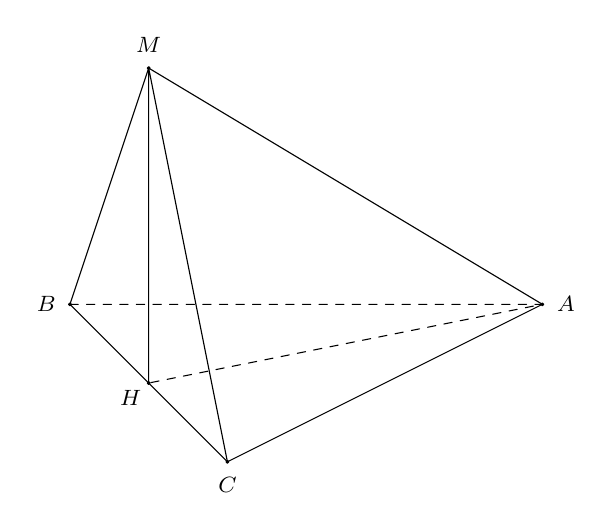
\begin{tikzpicture}[scale=1, font=\footnotesize, line join=round, line cap=round,>=stealth]
				\coordinate (A) at (6,0);
				\coordinate (B) at (0,0);
				\coordinate (C) at (2,-2);
				\coordinate (H) at (1,-1);
				\coordinate (M) at (1,3);
				\draw (B)--(M)--(A)--(C)--(B)--cycle;	
				\draw (H)--(M)--(C);			
				\draw[dashed](B)--(A)--(H);
				\foreach \p/\g in {A/0,B/180,C/-90,M/90,H/-140} \draw[fill] (\p) circle(.5pt) node [shift={(\g:.3)}] {$\p$};
			\end{tikzpicture}
		\end{center}
		Ta có $\overrightarrow{AB} = (2; 2; 0)$, $\overrightarrow{AC} = (-2; 2; 4) \Rightarrow \overrightarrow{AB} \cdot \overrightarrow{AC} = 0 \Rightarrow \triangle ABC$ suy ra $\triangle ABC$ vuông tại $A$.\\
		Gọi $H$ là hình chiếu vuông góc của điểm $M$ trên mặt phẳng $(ABC)$. Ta có\\
		$(MA, (ABC)) = (MA, HA) = \widehat{MAH}$.\\
		$(MB, (ABC)) = (MB, HB) = \widehat{MBH}$.\\
		$(MC, (ABC)) = (MC, HC) = \widehat{MCH}$.\\
		Theo giả thiết $\widehat{MAH} = \widehat{MBH} = \widehat{MCH} \Rightarrow \triangle MAH = \triangle MBH = \triangle MCH$ (g.c.g).\\
		Do đó $HA = HB = HC$ nên $H$ là tâm đường tròn ngoại tiếp $\triangle ABC$.\\
		Suy ra $H$ là trung điểm của $BC \Rightarrow H(1; 2; 2)$.\\
		Ta có $\left[\overrightarrow{AB}, \overrightarrow{AC}\right] = (8; -8; 8)$, chọn vec-tơ chỉ phương của đường thẳng $MH$ là $\overrightarrow{u}_{MH} = (1; -1; 1)$.\\
		PTĐT $MH$ có dạng:\\
		$$\heva{&x = 1 + t \\&	y = 2 - t \\&	z = 2 + t}\quad (t \in \mathbb{R}).$$
		Mặt cầu $(S)$ có tâm $I(3; 2; 3)$ và bán kính $R = \dfrac{\sqrt{2}}{2}$.
		\begin{center}
			\begin{tikzpicture}[scale=0.9, font=\footnotesize, line join=round, line cap=round,>=stealth]
				\coordinate (I) at (0,0);
				\coordinate (B) at (2,0);
				\coordinate (N) at ($(I)!1!-100:(B)$);
				\draw (I)circle (2);
				\coordinate (M) at ($(I)!1.5!(N)$);
				\coordinate (c) at ($(M)!1!-90:(I)$);
				\coordinate (d) at ($(c)!1.7!(M)$);
				\draw (c)--(d) (I)--(M);	
				\foreach \p/\g in {I/90,M/-95,N/-50} \draw[fill] (\p) circle(.5pt) node [shift={(\g:.3)}] {$\p$};
			\end{tikzpicture}
		\end{center}
		Gọi $K(1+t; 2-t; 2+t)$ là hình chiếu vuông góc của điểm $I$ trên đường thẳng $MH$.\\
		Ta có $\overrightarrow{IK} = (t-2; -t-1; t-1)$, $\overrightarrow{u}_{MH} = (1; -1; 1)$\\
		Do $IK \perp MH$ nên $\overrightarrow{IK} \cdot \overrightarrow{u}_{MH} = 0$, ta được $t = 1$. Khi đó $K(2; 1; 3)$ và $IK = \sqrt{2}$\\
		Do $IK > R$ nên đường thẳng $MH$ không cắt mặt cầu.\\
		Ta có $MN \geq \mathrm{d}(I, MH) - IN = IK - IN = \dfrac{\sqrt{2}}{2}.$
	}
\end{ex}
\begin{ex}%[2H5C3-3]
	Trong KG $Oxyz$, cho điểm $A(1;2;-3)$ và mặt phẳng $(P)\colon 2x+2y-z+9=0$. Đường thẳng $d$ đi qua $A$ và có vec-tơ chỉ phương $\vec{u}=(3;4;-4)$ cắt $(P)$ tại điểm $B$. Điểm $M$ thay đổi trong $(P)$ sao cho $M$ luôn nhìn đoạn $AB$ dưới góc $90^\circ$. Khi độ dài $MB$ lớn nhất, đường thẳng $MB$ đi qua điểm nào trong các điểm sau?
	\choice{$J(-3;2;7)$}{$K(3;0;15)$}{$H(-2;-1;3)$}{$I(-1;-2;3)$}
	\loigiai{
		\begin{center}
			\begin{tikzpicture}[scale=1,>=stealth, font=\scriptsize, line join=round, line cap=round,declare function={R=2;goc=-30;k=0.3;gocbu=180-goc;}]
				\pgfmathsetmacro\R{R}
				\pgfmathsetmacro\r{R*cos(goc)}
				\pgfmathsetmacro\a{.2*R}
				\pgfmathsetmacro\b{.2*\r}
				\pgfmathsetmacro\m{\r *cos(-50)}
				\pgfmathsetmacro\n{\b *sin(-50)}
				\path
				(0,0) coordinate (E)
				(-4,-1.5) coordinate (M')
				(2.5,-1.5) coordinate (N)
				(R,0)coordinate (A1)
				(-R,0)coordinate (A')
				(E)+(goc:R)coordinate (C)
				(E)+(-180-goc:R)coordinate (C')
				(barycentric cs:C'=1,C=1)coordinate(F)
				($(M')!2!(F)$)coordinate(P)
				($(N)!2!(F)$)coordinate(Q)
				($(Q)+(0.5,0)$)coordinate(K)
				($(P)+(-2.1,0)$)coordinate(T)
				;
				\path (F);
				\pgfgetlastxy{\xf}{\yf}
				\path
				($(F)+(\m,\n)$) coordinate (B)
				($(B)!2!(F)$)coordinate(M)
				($(B)!2!(E)$)coordinate(A)
				($(B)!2.5!(E)$)coordinate(d)
				;
				\draw (E)circle(R);
				\draw[dashed] (A1) arc (0:180:\R cm and \a cm);
				\draw[dashed] (C) arc (0:180:\r cm and \b cm);
				\draw[dashed] (M)--(B)--(A);
				\draw[dashed] (E)--(F);
				\draw (K)--(Q)--(M')--(N)--(P)--(T);
				\draw[dashed] (K)--(T);	
				\draw (A)--(d)node[above right]{$d$};
				\draw (A1) arc (0:-180:\R cm and \a cm);
				\draw (C) arc (0:-180:\r cm and \b cm);
				%			\draw (H)--(M)--(H') (M)--(X);
				\foreach \p/\g in{E/15,F/-100,B/45,M/-90,A/20}
				\shade[shading=ball](\p)circle(.03)node[shift={(\g:.25)},scale=1]{$\p$};
			\end{tikzpicture}
		\end{center}
		Đường thẳng $d$ đi qua $A$ và có vec-tơ chỉ phương $\overrightarrow{u} = (3; 4; -4)$ có phương trình là 
		$$\dfrac{x-1}{3} = \dfrac{y-2}{4} = \dfrac{z+3}{-4}.$$ 
		Tính được giao điểm của $d$ và $(P)$ là $B = (-2; -2; 1)$.\\ Do $M$ luôn nhìn đoạn $AB$ dưới góc $90^\circ$ nên $M$ nằm trên mặt cầu $(S)$ đường kính $AB$.\\
		Gọi $E$ là trung điểm của $AB \Rightarrow E = \left(-\dfrac{1}{2}; 0; -1\right) \Rightarrow AE^2 = \dfrac{41}{4}$.\\
		$\Rightarrow (S)\colon x^2 + y^2 + z^2 + x + 2z - 9 = 0$.\\
		Lại do $M \in (P)$ nên $M$ nằm trên đường tròn giao tuyến của mặt phẳng $(P)$ và mặt cầu $(S)$, gọi là đường tròn $(C)$.\\
		Mặt khác $B$ là điểm cố định trên đường tròn $(C)$ nên độ dài $MB$ lớn nhất khi $MB$ là đường kính của đường tròn $(C)$.\\
		Gọi $F$ là tâm của $(C) \Rightarrow F$ là hình chiếu vuông góc của $E$ trên $(P)$.\\
		Đường thẳng $EF$ nhận vec-tơ pháp tuyến $\overrightarrow{n} = (2; 2; -1)$ của $(P)$ làm vec-tơ pháp tuyến. Suy ra $EF$ có phương trình
		$$ \dfrac{x + \frac{1}{2}}{2} = \dfrac{y}{2} = \dfrac{z + 1}{-1}.$$
		Từ đó ta tính được $F = \left( -\dfrac{5}{2}; -2; 0 \right)$ (là giao điểm của $(P)$ và $EF$).\\
		Vì $MB$ là đường kính của $(C)$ nên $M = (-3; -2; -1) \Rightarrow \overrightarrow{MB} = (1; 0; 2)$ là vec-tơ chỉ phương của đường thẳng $MB \Rightarrow$ PTĐT $MB$ là 
		$$\heva{&x=-2+t\\&y=-2\\&z=1+2t} \quad (t \in \mathbb{R}).$$
		Trong các điểm đã cho ở các phương án chỉ có điểm $I (-1; -2; 3)$  thuộc đường thẳng $MB$.	
	}
\end{ex}
\begin{ex}%[2H5C2-6]
	Trong KG $Oxyz$, cho mặt cầu $(S)$ có tâm $I(1;2;3)$ và có bán kính $r=2$. Xét đường thẳng $d \colon \heva{&x=1+t \\&	y=-mt \\&	z=(m-1)t }\quad
	(t \in \mathbb{R})$, $ m$ là tham số  thực. \\
	Giả sử $(P), (Q)$ là mặt phẳng chứa $d$ và tiếp xúc với $(S)$ lần lượt tại $M, N$. Khi đó đoạn $MN$ ngắn nhất hãy tính khoảng cách từ điểm $B(1;0;4)$ đến đường thẳng $d$.
	\choice{$\sqrt{5}$}{$\dfrac{5\sqrt{3}}{3}$}{$\dfrac{4\sqrt{237}}{21}$}{\True$\dfrac{4\sqrt{273}}{21}$}
	\loigiai{
		\begin{center}
			\begin{tikzpicture}[scale=0.9, font=\footnotesize, line join=round, line cap=round,>=stealth]
				\coordinate (I) at (0,0);
				\coordinate (N) at (2,0);
				\coordinate (M) at($(I)!1!120:(N)$);				
				\coordinate (c) at ($(M)!1!90:(I)$);
				\coordinate (d) at ($(N)!1!-90:(I)$);
				\coordinate (H) at (intersection of M--c and N--d);
				\draw (I)circle (2);
				\draw (I)--(M)--(H)--(N)--(I)--cycle;
				\draw (H)--(I);	
				\draw pic[draw,angle radius=2mm] {right angle = I--M--H};
				\draw pic[draw,angle radius=2mm] {right angle = H--N--I};
				\foreach \p/\g in {I/-90,M/120,N/0,H/70} \draw[fill] (\p) circle(.5pt) node [shift={(\g:.3)}] {$\p$};
			\end{tikzpicture}
		\end{center}
		Mặt phẳng thiết diện đi qua tâm $I, M, N$ cắt đường thẳng $d$ tại $H$.\\
		Suy ra $IH \perp d$, $\mathrm{d}(I, d) = IH$.\\
		Ta có 
		$$MN = 2MK = 2 \cdot \dfrac{MH \cdot MI}{IH} = 2 \cdot \dfrac{\sqrt{IH^2 - r^2} \cdot r}{IH} = \dfrac{4 \sqrt{IH^2 - 4}}{IH}.$$ 
		Đặt $x = IH > 2$, ta có hàm số $ f(x)= \dfrac{4 \sqrt{x^2 - 4}}{x}$. \\
		Ta có $f'(x) = \dfrac{4}{x^2 \sqrt{x^2 - 4}} > 0, \forall x > 2$, suy ra hàm số đồng biến trên $(2; +\infty)$.\\
		Do đó $MN_{\text{min}} \Leftrightarrow IH_{\text{min}}$.\\
		Ta có $\overrightarrow{u}_d = (1; -m; m-1)$, $A(1; 0; 0) \in d$, suy ra
		$$\mathrm{d}(I, d) = \dfrac{\left| \overrightarrow{u}_d, \overrightarrow{IA} \right|}{|\overrightarrow{u}_d|}=\dfrac{\sqrt{25m^2 - 20m + 17}}{\sqrt{2m^2 - 2m + 2}}.$$
		Xét hàm số $f(m) = \dfrac{25m^2 - 20m + 17}{2m^2 - 2m + 2}$ có bảng biến thiên là
		\begin{center}
			
\begin{tikzpicture}[>=stealth]
				\tkzTabInit[nocadre=false,lgt=1.5,espcl=2,deltacl=0.5]
				{$m$/.7 ,$f'(m)$/.7,$f(m)$/2}
				{$-\infty$ , $\frac{1}{5}$ , $3$ , $+\infty$}
				\tkzTabLine{ , - , $0$ , + , $0$ , - , }
				\tkzTabVar{+/$\frac{25}{2}$ , -/$\frac{25}{3}$, +/$13$ ,  -/$\frac{25}{2}$}
			\end{tikzpicture}	
		\end{center}
		
		Suy ra $IH_{\text{min}}$ khi $m = \dfrac{1}{5}$. Đường thẳng $d$ có phương trình là\\
		$$\heva{&x = 1 + t \\ &y = -\dfrac{1}{5}t \\ &z = -\dfrac{4}{5}t} \quad (t \in \mathbb{R}).$$
		Khoảng cách $\mathrm{d}(B, d) = \dfrac{\left| \overrightarrow{AB}, \overrightarrow{u}_d \right|}{|\overrightarrow{u}_d|} = \dfrac{\sqrt{416}}{\sqrt{42}} = \dfrac{4 \sqrt{273}}{21}$.
		
	}
\end{ex}
\begin{ex}%[2H5C2-5]
	Trong KG $Oxyz$, cho mặt phẳng $(P)\colon 2x+2y-z+9=0$ và điểm $A(1;2;-3)$. Đường thẳng $d$ đi qua $A$ và có véc-tơ  chỉ phương $\vec{u} = (3;4;-4)$ cắt $(P)$ tại $B$. Điểm $M$ thay đổi trên $(P)$ sao cho $M$ luôn nhìn đoạn $AB$ dưới một góc $90^\circ$. Độ dài đoạn $MB$ lớn nhất bằng
	\choice{$\dfrac{36}{\sqrt{5}}$}{$\sqrt{41}$}{$6$}{\True$\sqrt{5}$}
	\loigiai{
		PTĐT $d\colon \heva{&x = 1 + 3t\\&y = 2 + 4t\\&z = -3 - 4t}$ nên tọa độ điểm $B$ thỏa mãn hệ phương trình \\
		$\heva{&x = 1 + 3t\\&y = 2 + 4t\\&z = -3 - 4t\\&2x + 2y - z + 9 = 0} \Rightarrow 2(1 + 3t) + 2(2 + 4t) - (-3 - 4t) + 9 = 0 \Leftrightarrow t = -1 \Rightarrow B(-2; -2; 1)$.\\
		Do $M$ nhìn đoạn $AB$ dưới một góc $90^\circ$ nên $M$ thuộc mặt cầu $(S)$ có đường kính $AB = \sqrt{41}$. Lại do $M \in (P)$ nên $M$ thuộc đường tròn giao tuyến giữa mặt cầu $(S)$ và mặt phẳng $(P)$.\\
		Do $MB$ là một dây cung của đường tròn này nên $MB$ lớn nhất khi nó là đường kính của đường tròn giao tuyến giữa mặt cầu $(S)$ và mặt phẳng $(P)$. Gọi $I\left(-\dfrac{1}{2}; 0; -1\right)$ là trung điểm $AB$ thì $I$ là tâm mặt cầu $(S)$ và $\mathrm{d}(I; (P)) = 3$. Khi đó bán kính đường tròn giao tuyến là
		$$r = \sqrt{\left(\dfrac{AB}{2}\right)^2 - \mathrm{d}^2(I; (P))} = \sqrt{\dfrac{41}{4} - 9} = \dfrac{\sqrt{5}}{2}.$$
		Vậy $MB_{\text{max}} = 2r = \sqrt{5}$.
	}
\end{ex}
\begin{ex}%[2H5C2-5]
	Trong KG $Oxyz$, cho mặt cầu $(S)\colon (x-1)^2+(y+1)^2+z^2 = \dfrac{5}{6}$, mặt phẳng $(P)\colon x+y+z+1=0$ và đường thẳng $\Delta\colon \dfrac{x}{1} = \dfrac{y}{1} = \dfrac{z}{1}$. Điểm $M$ thay đổi trên đường tròn giao tuyến của $(P)$ và $(S)$. Giá trị lớn nhất của $\mathrm{d}(M; \Delta)$ là
	\choice{\True$\dfrac{3\sqrt{2}}{2}$}{$2\sqrt{2}$}{$\sqrt{2}$}{$\dfrac{\sqrt{2}}{2}$}
	\loigiai{
		Mặt cầu $(S)$ có tâm là $I(1; -1; 0)$ và bán kính $R = \dfrac{\sqrt{30}}{6}$.\\
		Ta có $\mathrm{d}(I; (P)) = \dfrac{1}{3} < R$. Khi đó bán kính đường tròn giao tuyến là 
		$$r = \sqrt{R^2 - d^2} = \sqrt{\dfrac{5}{6} - \dfrac{1}{3}} = \dfrac{\sqrt{2}}{2}.$$
		$\Delta$ qua $O$ và có véc-tơ  chỉ phương $\overrightarrow{a} = (1; 1; 1) \Rightarrow \overrightarrow{OI} = (1; -1; 0)$, $\left[\overrightarrow{OI}, \overrightarrow{a}\right] = (-1; -1; 2)$.\\
		Ta có
		$$\mathrm{d}(I; \Delta) = \dfrac{\left|\left[\overrightarrow{OI}, \overrightarrow{a}\right]\right|}{|\overrightarrow{a}|} = \dfrac{\sqrt{1 + 1 + 4}}{\sqrt{1 + 1 + 1}} = \sqrt{2}.$$
		Mặt khác $\Delta \perp (P)$, gọi $H$ là tâm của đường tròn $(C)$ giao tuyến của $(P)$ và $(S)$.\\
		Ta có $IH = \mathrm{d}$. Do đó $\mathrm{d}(M; \Delta)$ lớn nhất $\Leftrightarrow \mathrm{d}(M; \Delta) = r + \mathrm{d}(IH; \Delta) = r + \mathrm{d}(I; \Delta)$.\\
		Khoảng cách lớn nhất của $\mathrm{d}(M; \Delta) = \dfrac{\sqrt{2}}{2} + \sqrt{2} = \dfrac{3 \sqrt{2}}{2}$.
		
	}
\end{ex}
\begin{ex}%[2H5C3-2]
	Trong KG $Oxyz$, cho hình lăng trụ đứng $ABC.A'B'C'$ có $A(x_0; 0; 0)$, $B(-x_0; 0; 0)$, $C(0; 1; 0)$ và $B'(-x_0; 0; y_0)$ trong đó $x_0, y_0$ là các số thực dương và thỏa mãn $x_0 + y_0 = 4$. Khi khoảng cách giữa hai đường thẳng $AC'$ và $B'C$ lớn nhất thì bán kính $R$ của mặt cầu ngoại tiếp hình lăng trụ $ABC.A'B'C'$ bằng bao nhiêu?
	\choice{\True$\dfrac{\sqrt{29}}{2}$}{$\dfrac{29}{4}$}{$\dfrac{\sqrt{41}}{4}$}{$\dfrac{3\sqrt{6}}{2}$}
	\loigiai{
		\begin{center}
			\begin{tikzpicture}[scale=0.9, font=\footnotesize, line join=round, line cap=round,>=stealth]
				\def \h{5}
				
				% Define coordinates
				\coordinate (O) at (0,0);
				\coordinate (A) at (-1,-1);
				\coordinate (B) at (1,1);
				\coordinate (C) at (2.5,0); 
				\coordinate (O') at ($(O)+(0,\h)$);
				\coordinate (z) at ($(O)+(0,6.5)$);		
				\coordinate (A') at ($(A)+(0,\h)$);			
				\coordinate (B') at ($(B)+(0,\h)$);	
				\coordinate (C') at ($(C)+(0,\h)$);
				\coordinate (x) at ($(O)!1.4!(A)$);
				\coordinate (y) at ($(O)!1.4!(C)$);
				
				% Draw shapes and lines
				\draw (A)--(C)--(C')--(B')--(A')--(A)--cycle;
				\draw (A')--(C');	
				\draw[dashed] (A)--(B)--(C);
				\draw[dashed] (C)--(O)--(O');
				\draw[dashed] (B)--(B');
				\draw[->](A)--(x);
				\draw[->](C)--(y);
				\draw[->](O')--(z);
				
				% Draw points and labels
				\foreach \p/\g in {A/170,B/20,C/-90,A'/180,B'/90,C'/0,x/-90,y/-90,z/120} 
				\draw[fill] (\p) circle(.5pt) node [shift={(\g:.3)}] {$\p$};
			\end{tikzpicture}
		\end{center}
		Vì $ABB'A'$, $ACC'A'$, $BCC'A'$ là các hình chữ nhật nên ta tính được tọa độ các đỉnh còn lại của hình lăng trụ $A'(x_0; 0; y_0), C'(0; 1; y_0)$.\\
		Ta có
		$\overrightarrow{AC'} = (-x_0; 1; y_0), \overrightarrow{B'C'} = (x_0; 1; -y_0)$ và $\overrightarrow{CC'} = (0; 0; y_0)$. Suy ra\\
		$$\mathrm{d}(AC', B'C') = \dfrac{\left|\left[\overrightarrow{AC'}, \overrightarrow{B'C'}\right].\overrightarrow{CC'}\right|}{\left|\left[\overrightarrow{AC'}, \overrightarrow{B'C'}\right]\right|} = \dfrac{|x_0 y_0|}{\sqrt{x_0^2 + y_0^2}} = \dfrac{\sqrt{(x_0 y_0)^2}}{\sqrt{(x_0 + y_0)^2 - 2x_0 y_0}}.$$
		Đặt $t = x_0 y_0 \leq \left(\dfrac{x_0 + y_0}{2}\right)^2 = 4 \Rightarrow t \in [0; 4]$.\\
		Xét $f(t) = \dfrac{t^2}{16 - 2t} \Rightarrow f'(t) = \dfrac{32t - 2t^2}{(16 - 2t)^2}$.\\
		Cho $f'(t) = 0 \Rightarrow \heva{&t = 0\\&t = 16.}$
		\begin{center}
			\begin{tikzpicture}[font=\footnotesize, line join=round, line cap=round, >=stealth,yscale=.6,xscale=1]
				\def \x{8}
				\draw 
				(-.5,.5) rectangle +(\x,-5)
				(-.5,-.5)--+(0:\x) (-.5,-1.5)--+(0:\x) (.5,.5)--+(-90:5);
				\path
				(0,0) node{$t$}
				(0,-1) node{$f'(t)$}
				(0,-3) node{$f(t)$}
				(1,0) node{$-\infty$}
				(3,0) node{$0$}
				(3,-4) node(b){$ $}
				(5,0) node{$4$}
				(5,-2) node(c){$ $}
				(7,0) node{$+\infty$}
				(4,-1) node{$+$};
				\draw[->] (b)--(c);
				\draw[pattern=north east lines] (0.5,-4.5) rectangle (3,-0.5);
				\draw[pattern=north east lines] (5,-4.5) rectangle (7.5,-0.5);
			\end{tikzpicture}
		\end{center}
		Giá trị lớn nhất của $\mathrm{d}(AC', B'C')$ bằng $f(4)$ nên $x_0 y_0 = 4\quad (1)$.\\
		Mặt khác $x_0 + y_0 = 4 \quad (2)$.\\
		Từ (1) và (2) ta có $x_0 = y_0 = 2$.\\
		Khi đó, $AB = 4, AC = BC = \sqrt{5}$ và chiều cao hình lăng trụ là $h = CC' = 2$.\\
		Ta có $r = \dfrac{AB \cdot AC \cdot BC}{4S_{\triangle ABC}} = \dfrac{5}{2}$ là bán kính đường tròn ngoại tiếp đáy $\triangle ABC$.\\
		Vậy $R = \sqrt{r^2 + \left(\dfrac{h}{2}\right)^2} = \sqrt{\left(\dfrac{5}{2}\right)^2 + \left(\dfrac{2}{2}\right)^2} = \dfrac{\sqrt{29}}{2}$.	
	}
\end{ex}
\begin{ex}%[2H5C2-3]
	Trong KG $Oxyz$, cho hai điểm $A(2;1;-2)$, $B(5;1;1)$ và mặt cầu $(S)\colon x^2 + y^2 + z^2 + 6y + 12z + 9 = 0$. Xét đường thẳng $d$ đi qua $A$ và tiếp xúc với $(S)$ sao cho khoảng cách từ $B$ đến $d$ nhỏ nhất. Phương trình của đường thẳng $d$ là
	\choice{	$\heva{&x=2\\&y=1+t\\&z=-2+2t}$}
	{$\heva{&x=2\\&y=1-4t\\&z=-2+t}$	}
	{\True$\heva{&x=2+2t\\&y=1-2t\\&z=-2+t}$}
	{$\heva{&x=2+t\\&y=1+4t\\&z=-2-t}$}
	\loigiai{
		Mặt cầu $(S)$ có tâm $I(0; -3; -6)$ và bán kính $R = \sqrt{3^2 + 6^2 - 9} = 6$.\\
		Vì $IA = R$ nên $A \in (S) \Rightarrow d$ đi qua $A$ và vuông góc với $IA \Rightarrow d$ nằm trong $(P)$ là mặt phẳng đi qua $A$ và vuông góc với $IA$. Ta có $(P)\colon x + 2y + 2z = 0$.\\
		Mặt khác, ta luôn có
		$$\mathrm{d}(B, d) \geq \mathrm{d}(B, (P)) = 3.$$
		Đẳng thức xảy ra $\Leftrightarrow d$ là hình chiếu của đường thẳng $AB$ trên $(P)$.\\
		Ta tìm hình chiếu $H$ của $B$ trên $(P)$.\\
		Gọi $\Delta$ là đường thẳng qua $B$ và vuông góc với $(P)$ nên có phương trình
		$$ \Delta\colon \dfrac{x - 5}{1} = \dfrac{y - 1}{2} = \dfrac{z - 1}{2}.$$
		Vì $H$ là giao điểm của $\Delta$ và $(P)$ nên tọa độ $H$ là nghiệm của hệ.\\
		$\heva{&\dfrac{x - 5}{1} = \dfrac{y - 1}{2} = \dfrac{z - 1}{2}\\&x + 2y + 2z = 0} \Leftrightarrow \heva{&x = 4\\&y = -1\\&z = -1} \Rightarrow H(4; -1; -1)$.\\
		$\Rightarrow \overrightarrow{AH} = (2; -2; 1)$.\\
		Do đó, $d$ là đường thẳng đi qua hai điểm $A$ và $H$ nên có phương trình
		$$\heva{&x = 2 + 2t\\&y = 1 - 2t\\&z = -2 + t.}$$
	}
\end{ex}
\Closesolutionfile{ans}
% \indapan{10}{ans/ans-2-C3B5CD5}

\TNSA
\Opensolutionfile{ans}[ans/ans-C5B3CD6-KQ]
\begin{ex}%[2H5C2-3]
	Trong KG $Oxyz$, cho đường thẳng $d\colon \dfrac{x-2}{1} = \dfrac{y+1}{2} = \dfrac{z}{3}$ và hai điểm $A(2;0;3)$, $B(2;-2;-3)$. Biết điểm $M(x_0;y_0;z_0)$ thuộc $d$ thỏa mãn $MA^4 + MB^4$ nhỏ nhất. Tìm $x_0$.
	\shortans{$2$}
	\loigiai{
		Gọi $I$ là trung điểm của $AB$. Khi đó ta có
		\allowdisplaybreaks
		\begin{eqnarray*}
			MA^4 + MB^4 &= &\left(MA^2 + MB^2\right)^2 - 2MA^2 \cdot MB^2 = \left(2MI^2 + \dfrac{AB^2}{2}\right)^2 - 2\left(MI^2 - \dfrac{AB^2}{4}\right)^2\\
			&=& 4MI^4 + 2MI^2 AB^2 + \dfrac{AB^4}{4} - 2MI^4 + MI^2 AB^2 - \dfrac{AB^4}{8}\\
			&=&2MI^4 + 3MI^2 AB^2 + \dfrac{AB^4}{4} = 2\left(MI^2 + \dfrac{3AB^2}{4}\right)^2 - \dfrac{7}{10} AB^4.
		\end{eqnarray*}
		Do đó, $MA^4 + MB^4$ đạt giá trị nhỏ nhất khi $MI$ nhỏ nhất $\Leftrightarrow M$ là hình chiếu vuông góc của $I$ lên $d$.\\
		Điểm $I (2; -1; 0)$. Lấy $M (2 + t; -1 + 2t; 3t) \in d$. Ta có $\overrightarrow{IM} = (t; 2t; 3t)$. Suy ra
		$$\overrightarrow{IM} \perp \overrightarrow{u}_d \Leftrightarrow \overrightarrow{IM} \cdot \overrightarrow{u}_d = 0 \Leftrightarrow t + 4t + 9t = 0 \Leftrightarrow t = 0.$$
		Suy ra $M \equiv I$.\\
		Vậy $x_0 = 2$.	
	}
\end{ex}
\begin{ex}%[2H5C2-5]
	Trong KG $Oxyz$, cho điểm $A(1;1;1)$ và mặt phẳng $(P)\colon x+2y=0$. Gọi $\Delta$ là đường thẳng đi qua $A$, song song với $(P)$ và cách điểm $B(-1;0;2)$ một khoảng ngắn nhất. Gọi $\overrightarrow{u}=(6;b;c)$ là một véc-tơ  chỉ phương của đường thẳng $\Delta$. Tính $M=b^2+c^2$.
	\shortans{$34$}
	\loigiai{
		Gọi $(Q)$ chứa $\Delta$ và song song với $(P)$. Suy ra $(Q)$ có phương trình
		$$x - 1 + 2(y - 1) = 0 \Leftrightarrow x + 2y - 3 = 0.$$
		Khi đó $\mathrm{d}(B; \Delta)_{\text{min}} = BH$ với $H$ là hình chiếu của $B$ lên mặt phẳng $(Q)$.\\
		Đường thẳng $BH$ đi qua $B$, vuông góc với mặt phẳng $(Q)$ có phương trình 
		$$\heva{&x = -1 + t\\&y = 2t\\&z = 2}, t \in \mathbb{R}.$$
		Tọa độ giao điểm $H$ của đường thẳng $BH$ và mặt phẳng $(Q)$ là nghiệm của hệ
		$$\heva{&x = -1 + t\\&y = 2t\\&z = 2\\&x + 2y - 3 = 0.}$$
		Giải hệ trên ta được $H\left(-\dfrac{1}{5}; \dfrac{8}{5}; 2\right)$.\\
		Do đó $\Delta$ là đường thẳng $AH$ có $\overrightarrow{AH} = \left(\dfrac{6}{5}; -\dfrac{3}{5}; -1\right)$.\\
		Suy ra $\overrightarrow{u} = (6; -3; -5)$ cũng là một véc-tơ  chỉ phương của $\Delta$.\\
		Suy ra $b=-3$, $c=-5$. Vậy $b^2+c^2=34$.\\
		\textbf{Cách 2}\\
		Gọi $\overrightarrow{u} = (a; b; c), a^2 + b^2 + c^2 > 0$ là một véc-tơ  chỉ phương của $\Delta$.\\
		Mặt phẳng $(P)\colon x + 2y = 0$ có một véc-tơ  pháp tuyến là $\overrightarrow{n} = (1; 2; 0)$.\\
		$\Delta$ song song với $(P)$ nên $\overrightarrow{n} \cdot \overrightarrow{u} = 0 \Leftrightarrow a + 2b = 0 \Leftrightarrow a = -2b$. $\Rightarrow \overrightarrow{u} = (-2b; b; c)$.\\
		Ta có $\overrightarrow{AB} = (-2; -1; 1), \left[\overrightarrow{u}, \overrightarrow{AB}\right] = (b + c; 2b - 2c; 4b)$.\\
		Khoảng cách từ $B(-1; 0; 2)$ đến $\Delta$ là
		$$\mathrm{d}(B, \Delta) = \dfrac{\left|\left[\overrightarrow{u}, \overrightarrow{AB}\right]\right|}{|\overrightarrow{u}|} = \sqrt{\dfrac{21b^2 - 6bc + 5c^2}{5b^2 + c^2}}.$$
		Nếu $c = 0 \Rightarrow b \neq 0 \Rightarrow \mathrm{d}(B, \Delta) = \sqrt{\dfrac{21}{5}}$.\\
		Nếu $c \neq 0$ thì  $\mathrm{d}(B, \Delta) = \sqrt{\dfrac{21\left(\dfrac{b}{c}\right)^2 - 6 \dfrac{b}{c} + 5}{5 \left(\dfrac{b}{c}\right)^2 + 1}}$. \\
		Đặt $t = \dfrac{b}{c}$, ta được $\mathrm{d}(B, \Delta) = \sqrt{\dfrac{21t^2 - 6t + 5}{5t^2 + 1}}$.\\
		Xét $f(t) = \dfrac{21t^2 - 6t + 5}{5t^2 + 1}, f'(t) = \dfrac{30t^2 - 8t - 6}{(5t^2 + 1)^2}$.\\
		$f'(t) = 0 \Leftrightarrow \heva{&t = -\dfrac{1}{3}\\&t = \dfrac{3}{5}}$.
		\begin{center}
			
\begin{tikzpicture}[>=stealth]
				\tkzTabInit[nocadre=false,lgt=1.5,espcl=2,deltacl=0.5]
				{$t$/.7 ,$f'(t)$/.7,$f(t)$/2}
				{$-\infty$ , $-\frac{1}{3}$ , $\frac{3}{5}$ , $+\infty$}
				\tkzTabLine{ , + , $0$ , - , $0$ , + , }
				\tkzTabVar{-/$\frac{21}{5}$ , +/$6$, -/$\frac{16}{5}$ ,  +/$\frac{21}{5}$}
			\end{tikzpicture}
		\end{center}
		Dựa vào bảng biến thiên ta có giá trị nhỏ nhất của $f(t)$ bằng $\dfrac{16}{5}$ khi $t = \dfrac{3}{5}$.\\
		$\Rightarrow (\mathrm{d}(B, \Delta))_{\text{min}} = \dfrac{4}{\sqrt{5}}$ khi $t = \dfrac{3}{5} \Rightarrow \dfrac{b}{c} = \dfrac{3}{5}$.\\
		Chọn $b = -3, c = -5 \Rightarrow a = 6$. Suy $\Delta$ nhận véc-tơ  $\overrightarrow{u} = (6; -3; -5)$ làm véc-tơ  chỉ phương.\\
		Vậy $b^2+c^2=34$.	
	}
\end{ex}

\begin{ex}%[2H5C2-5]
	Trong KG $Oxyz$, cho hai điểm $A(-3;0;1)$, $B(1;-1;3)$ và mặt phẳng $(P): x-2y+2z-5=0$. Đường thẳng $d$ đi qua $A$, song song với mặt phẳng $(P)$ sao cho khoảng cách từ $B$ đến $d$ nhỏ nhất. Gọi $\overrightarrow{u}=(26;a;b)$ là một véc-tơ chỉ phương của $d$. Tính $a+b$.
	\shortans{$9$}
	\loigiai{
		\begin{center}
			\begin{tikzpicture}[scale=0.9, font=\footnotesize, line join=round, line cap=round,>=stealth]
				\def \m{-1}
				\def \n{-2}		
				% Define coordinates
				\coordinate (A) at (0,0);
				\coordinate (B1) at (5,0);
				\coordinate (D) at (1.5,1.8);
				\coordinate (C) at (6.5,1.8); 
				\coordinate (Q) at (0.2,0.2); 	
				\coordinate (A') at ($(A)+(\m,\n)$);
				\coordinate (B') at ($(B1)+(\m,\n)$);	
				\coordinate (C') at ($(C)+(\m,\n)$);		
				\coordinate (D') at ($(D)+(\m,\n)$);
				\coordinate (P) at ($(Q)+(\m,\n)$);
				\coordinate (H) at (2,1);
				\coordinate (B) at (2,4);
				\coordinate (K) at (4,1);
				\coordinate (M) at (2,0.2);
				\coordinate (N) at ($(M)!1.5!(K)$);	
				\coordinate (d) at ($(M)!1.1!(K)$);	
				\coordinate (E) at (intersection of H--B and C--D);	
				\coordinate (F) at (intersection of K--B and C--D);	
				% Draw shapes and lines
				\draw (E)--(D)--(A)--(B1)--(C)--(F);
				\draw (H)--(B)--(K)--cycle;
				\draw (A')--(B')--(C')--(D')--cycle;
				\draw (M)--(N);	
				\draw[dashed] (E)--(F);
				\begin{scope}
					\clip (B1)--(A)--(D);
					\draw (A) circle (9mm);
				\end{scope}
				\begin{scope}
					\clip (B')--(A')--(D');
					\draw (A') circle (9mm);
				\end{scope}
				\draw pic[draw,angle radius=2mm] {right angle = K--H--B};
				\draw pic[draw,angle radius=2mm] {right angle = H--K--M};
				% Draw points and labels
				\foreach \p/\g in {B/-160,H/190,K/-45} 
				\draw[fill] (\p) circle(.5pt) node [shift={(\g:.3)}] {$\p$};
				\foreach \p/\g in {d/70,P/10,Q/10} 
				\draw (\p) node [shift={(\g:.3)}] {$\p$};
			\end{tikzpicture}
		\end{center}
		Ta thấy rằng $d$ đi qua $A$ và $d$ song song với $(P)$ nên $d$ luôn nằm trong mặt phẳng $(Q)$ qua $A$ và $(Q) \parallel (P)$. Như vậy bây giờ ta chuyển về xét trong mặt phẳng $(Q)$ để thay thế cho $(P)$. Ta lập được phương trình mặt phẳng $(Q)\colon x - 2y - 2z + 1 = 0$.\\
		Gọi $H, K$ lần lượt là hình chiếu của $B$ lên $(Q)$ và $d$. Ta tìm được $H\left(-\dfrac{1}{9}; \dfrac{11}{9}; \dfrac{7}{9}\right)$.\\
		Ta luôn có  $d(B; d) = BK \geq BH$ nên khoảng cách từ $B$ đến $d$ bé nhất bằng $BH$.\\
		Đường thẳng $d$ bây giờ đi qua $A, H$ nên có véc-tơ  chỉ phương $\overrightarrow{u}=(26;11;-2)$.\\
		Suy ra $a=11$, $b=-2$. Vậy $a+b=9$.	
	}
\end{ex}
\begin{ex}%[2H5C2-6]%[ID]
	Trong KG $Oxyz$, cho điểm $A(0 ; 3 ;-2)$. Xét đường thẳng $d$ thay đổi song song với $Oz$ và cách $Oz$ một khoảng bằng $2$. Khi khoảng cách từ $A$ đến $d$ nhỏ nhất, biết $d$ đi qua điểm $M(a;b;c)$ sao cho $a$, $b$, $c$ lập thành một cấp số cộng. Tính $a^2+b^2-c^2$.
	\shortans{$-12$}
	\loigiai{
		Vì $d$ song song với $Oz$ và cách $Oz$ một khoảng bằng $2$ nên $d$ thuộc mặt trụ trục $Oz$ và bán kính bằng $2$.\\
		Có $H(0 ; 0 ;-2)$ là hình chiếu vuông góc của $A(0 ; 3 ;-2)$ trên $Oz$.\\
		Có $\overrightarrow{HA}=(0 ; 3 ; 0) \Rightarrow H A=3$ nên $A$ nằm ngoài mặt trụ.\\
		Gọi $(P)$ là mặt phẳng qua $A$ và vuông góc với $Oz$.\\
		$M$ là hình chiếu vuông góc của $A$ trên $d$.\\
		Gọi $K$ là giao điểm của $AH$ và mặt trụ ($K$ nằm giữa $A$ và $H$).\\
		Dễ thấy $D(A ; d)=A M \geq A K$; $A K=A H-D(A ; d)=1$.\\
		Dấu bằng xảy ra khi và chỉ khi $M \equiv K$.\\
		Khi đó ta có $\overrightarrow{H K}=\dfrac{2}{3} \overrightarrow{H A} \Rightarrow K(0 ; 2 ;-2) \Rightarrow d\colon \heva{&x=0 \\ &y=2 \\ &z=-2+t} (t \in \mathbb{R})$.\\
		Vậy điểm $M \in d$ sẽ là $M(0;2;4)$ suy ra $a^2+b^2-c^2=-12$.
	}
\end{ex}

\begin{ex}%[2H5C2-7]%[ID]
	Trong KG $Oxyz$, đường thẳng $\Delta$ đi qua điểm $M(3 ; 1 ; 1)$, nằm trong mặt phẳng $(\alpha)\colon x+y-z-3=0$ và tạo với đường thẳng $d\colon \heva{&x=1 \\ &y=4+3 t \\ &z=-3-2 t}$ một góc nhỏ nhất. Biết điểm $N(a;b;2) \in d$, tính $\dfrac{4b}{a}$.
	\shortans{$-1{,}5$}
	\loigiai{
		\begin{itemize}
			\item \textbf{Cách 1.}\\
			Gọi $d'$ là hình chiếu vuông góc của $d$ lên $(\alpha)$, khi đó góc $\left(d, d'\right)$ là góc nhỏ nhất trong các góc tạo bởi $d$ với đường thẳng bất kỳ trong $(\alpha)$.\\
			$d$ có véc-tơ chỉ phương $\overrightarrow{u}_d=(0 ; 3 ;-2)$, $(\alpha)$ có véc-tơ pháp tuyến $\overrightarrow{n}_\alpha=(1 ; 1 ;-1)$.\\
			Gọi $\overrightarrow{n}_\beta$ là véc-tơ pháp tuyến của mặt phẳng $(\beta)$ tạo bởi $d$ và $d'$ thì $\overrightarrow{n}_\beta \perp \overrightarrow{u}_d$, $\overrightarrow{n}_\beta \perp \overrightarrow{n}_\alpha$ ta chọn $\overrightarrow{n}_\beta=\left[\overrightarrow{n}_\alpha, \overrightarrow{u}_d\right]=(1 ; 2 ; 3)$.\\
			Gọi $\overrightarrow{u}_{d'}$ là véc-tơ chỉ phương của $d'$ thì $\overrightarrow{u}_{d'} \perp \overrightarrow{n}_\alpha, \overrightarrow{u}_{d'} \perp \overrightarrow{n}_\beta$, ta chọn $\overrightarrow{u}_{d'}=\left[\overrightarrow{n}_\alpha, \overrightarrow{n}_\beta\right]=(5 ;-4 ; 1)$.\\
			Đường thẳng $\Delta$ song song hoặc trùng với $d'$ nên có véc-tơ chỉ phương $\overrightarrow{u}_{\Delta}=\overrightarrow{u}_{d'}=(5 ;-4 ; 1)$.\\
			Vậy PTTS của đường thẳng $\Delta$ là $\heva{&x=3+5t\\&y=1-4t\\&z=1+t.} (t \in \mathbb{R})$\\
			Do $N(a;b;2) \in \Delta \Leftrightarrow \heva{&a=3+5t\\&b=1-4t\\&2=1+t} \Leftrightarrow\heva{&a=8\\&b=-3\\&t=1.} $ nên $\dfrac{4b}{a}=-1{,}5$.
			\item \textbf{Cách 2.}\\
			$d$ có véc-tơ chỉ phương $\overrightarrow{u}_d=(0 ; 3 ;-2)$, $(\alpha)$ có véc-tơ pháp tuyến $\overrightarrow{n}_\alpha=(1 ; 1 ;-1)$.\\
			Giả sử $\Delta$ có véc-tơ chỉ phương $\overrightarrow{u}_{\Delta}=(a ; b ; c),\left(a^2+b^2+c^2>0\right)$.\\
			Do $\Delta \subset(\alpha)$ ta có $\overrightarrow{n}_\alpha \cdot \overrightarrow{u}_{\Delta}=0 \Leftrightarrow a+b-c=0 \Leftrightarrow c=a+b$.
			Gọi $\varphi$ là góc giữa $\Delta$ và $d$, $\varphi \in\left[0 ; \dfrac{\pi}{2}\right]$, khi đó
			$$
			\cos \varphi=\left|\cos \left(\overrightarrow{u}_{\Delta}, \overrightarrow{u}_d\right)\right|=\dfrac{|3 b-2 c|}{\sqrt{13} \cdot \sqrt{a^2+b^2+c^2}}=\dfrac{|b-2 a|}{\sqrt{13} \cdot \sqrt{2 a^2+2 b^2+2 a b}}
			$$
			Góc $\varphi$ nhỏ nhất khi và chỉ khi $\cos \varphi$ lớn nhất, ta xét các trường hợp
			\begin{itemize}
				\item \textbf{Trường hợp 1.} Nếu $a=0$ ta được $\cos \varphi=\dfrac{1}{\sqrt{26}}$.
				\item \textbf{Trường hợp 2.} Nếu $a \neq 0$ ta được $\cos \varphi=\dfrac{|t-2|}{\sqrt{26\left(t^2+t+1\right)}}$, $\left(t=\dfrac{b}{a}\right)$.\\
				Ta có $26 \cos ^2 \varphi=\dfrac{t^2-4 t+4}{t^2+t+1}$, đặt $f(t)=\dfrac{t^2-4 t+4}{t^2+t+1}, t \in \mathbb{R}$, có
				$$	f'(t)=\dfrac{5 t^2-6 t-8}{\left(t^2+t+1\right)^2},\ f'(t)=0 \Leftrightarrow\hoac{&t=2 \\&	t=-\dfrac{4}{5}.}$$
				Bảng biến thiên của hàm số $f(t)$ như sau
				\begin{center}
					
\begin{tikzpicture}[>=stealth]
						\tkzTabInit[nocadre=false,lgt=1.2,espcl=2,deltacl=0.5]{$t$/1.2 ,$f'(t)$/.7,$f(t)$/2}
						{$-\infty$ , $-\dfrac{4}{5}$ , $2$ , $+\infty$}
						\tkzTabLine{ , + , $0$ , - , $0$ , + , }
						\tkzTabVar{-/$1$ , +/$\dfrac{28}{3}$ , -/$\dfrac{2}{3}$ , +/$1$}
					\end{tikzpicture}
				\end{center}
				Do $\cos \varphi \geq 0$ nên $\cos \varphi$ lớn nhất khi $f(t)$ lớn nhất, từ bảng biến thiên ta được $\max\limits_{t \in \mathbb{R}} f(t)=f\left(-\dfrac{4}{5}\right)$.\\
				Khi đó $\dfrac{b}{a}=-\dfrac{4}{5} \Leftrightarrow 5 b=-4 a$, chọn $a=5 \Rightarrow b=-4$ và ta được $c=1$.\\
				Đường thẳng $\Delta$ có véc-tơ chỉ phương $\overrightarrow{u}_{\Delta}=(5 ;-4 ; 1)$.\\
				Vậy PTTS của đường thẳng $\Delta$ là $\heva{&x=3+5t\\&y=1-4t\\&z=1+t.} (t \in \mathbb{R})$\\
				Do $N(a;b;2) \in \Delta \Leftrightarrow \heva{&a=3+5t\\&b=1-4t\\&2=1+t} \Leftrightarrow\heva{&a=8\\&b=-3\\&t=1} $ nên $\dfrac{4b}{a}=-1{,}5$.
			\end{itemize}
		\end{itemize}
	}
\end{ex}

\begin{ex}%[2H5C2-3]
	Trong không gian với hệ tọa độ $O x y z$, cho đường thẳng $(d)\colon \heva{&x=-1+2 t \\ &y=1-t \\ &z=2 t}$ và hai điểm $A(1 ; 5 ; 0)$, $B(3 ; 3 ; 6)$. Gọi $M(a ; b ; c)$ là điểm trên $(d)$ sao cho chu vi tam giác $M A B$ đạt giá trị nhỏ nhất. Tính $P=a+b+c$.
	\shortans{$3$}
	\loigiai{
		Ta có $M \in d \Rightarrow M(-1+2 t ; 1-t ; 2 t)$.\\
		Chu vi tam giác $M A B$ là $A M+B M+A B$.\\
		Vì $A B$ là hằng số nên chu vi nhỏ nhất khi $A M+B M$ nhỏ nhất.\\
		Ta có $\overrightarrow{A M}(2 t-2 ;-t-4 ; 2 t)$, $\overrightarrow{B M}(2 t-4 ;-t-2 ; 2 t-6)$.
		$$
		A M+B M=\sqrt{9 t^2+20}+\sqrt{9 t^2-36 t+56}=\sqrt{(3 t)^2+(2 \sqrt{5})^2}+\sqrt{(6-3 t)^2+(2 \sqrt{5})^2}
		$$
		Đặt $\overrightarrow{u}=(3 t ; 2 \sqrt{5})$, $\overrightarrow{v}=(6-3 t ; 2 \sqrt{5}) \Rightarrow \overrightarrow{u}+\overrightarrow{v}=(6 ; 4 \sqrt{5})$.\\
		Áp dụng bất đẳng thức véc-tơ  $|\overrightarrow{u}|+|\overrightarrow{v}| \geq|\overrightarrow{u}+\overrightarrow{v}|$.\\
		Dấu bằng xảy ra khi $\overrightarrow{u}$, $\overrightarrow{v}$ cùng hướng.\\
		Ta có $A M+B M=|\overrightarrow{u}|+|\overrightarrow{v}| \geq|\overrightarrow{u}+\overrightarrow{v}|=\sqrt{6^2+(4 \sqrt{5})^2}=2 \sqrt{29}$.\\
		Do đó $A M+B M$ nhỏ nhất khi tồn tại số $k$ dương sao cho $$\overrightarrow{u}=k \overrightarrow{v} \Leftrightarrow\heva{&3 t=k(6-3 t) \\ &2 \sqrt{5}=2 \sqrt{5} k}\Leftrightarrow\heva{&t=1 \\ &k=1.}$$
		Khi đó $M(1 ; 0 ; 2)$ nên $P=a+b+c=1+0+2=3$.
	}
\end{ex}

\begin{ex}%[2H5C2-5]%[ID]
	Trong không gian với hệ tọa độ $O x y z$, cho tứ diện $A B C D$ có $A(-1 ; 1 ; 6)$, $B(-3 ;-2 ;-4)$, $C(1 ; 2 ;-1)$, $D(2 ;-2 ; 0)$. Điểm $M(a ; b ; c)$ thuộc đường thẳng $C D$ sao cho tam giác $A B M$ có chu vi nhỏ nhất. Tính $T=a+b+c$.
	\shortans{$1$}
	\loigiai{
		Gọi $C_{A B M}$ là chu vi của tam giác $A B M$.\\
		$ \overrightarrow{A B}=(-2 ;-3 ;-10) \Rightarrow A B=\sqrt{113} $.\\
		$ \overrightarrow{A B}=(-2 ;-3 ;-10)$, $\overrightarrow{C D}=(1 ;-4 ; 1) \Rightarrow \overrightarrow{A B} \cdot \overrightarrow{C D}=-2+12-10=0 \Rightarrow A B \perp C D$.
		Gọi $(P)$ là mặt phẳng chứa đường thẳng $A B$ và vuông góc với đường thẳng $C D$.\\ $H$ là giao điểm của $(P)$ và đường thẳng $C D$.\\
		Phương trình mặt phẳng $(P)$ qua $A(-1 ; 1 ; 6)$ có véc-tơ pháp tuyến $\overrightarrow{C D}=(1 ;-4 ; 1)$ là
		$$	x-4 y+z-1=0.$$
		PTĐT $C D\colon \heva{&x=1+t \\ &y=2-4 t \\ &z=-1+t.}$\\
		$ H \in C D \Leftrightarrow H(1+t ; 2-4 t ;-1+t)$.\\
		$H \in(P) \Leftrightarrow 1+t-4(2-4 t)-1+t-1=0 \Leftrightarrow t=\dfrac{1}{2} \Leftrightarrow H\left(\dfrac{3}{2} ; 0 ;-\dfrac{1}{2}\right)$.\\
		Với mọi $ M \in C D$, ta có $\heva{&A M \geq A H \\ &B M \geq B H} \Rightarrow A M+B M \geq A H+B H$.\\
		$$	\mathrm{C}_{A B M}=A B+A M+B M \geq \sqrt{113}+A H+B H,\ \forall M \in C D \text {. }
		$$
		Suy ra $\min \mathrm{C}_{A B M}=\sqrt{113}+A H+B H$, đạt được $M \equiv H \Leftrightarrow M\left(\dfrac{3}{2} ; 0 ;-\dfrac{1}{2}\right)$.\\
		Vậy $T=a+b+c=1$.
	}
\end{ex}
\Closesolutionfile{ans}
% \indapan{6}{ans/ans-C5B3CD6-KQ}